\documentclass[]{article}

\def\nno{\nonumber}
\def\bfE{\mbox{\boldmath$E$}}
\def\bfG{\mbox{\boldmath$G$}}
\def \p{\partial}
\usepackage{epsfig, color}
\usepackage{color,graphicx}
\usepackage{amsfonts}
\usepackage{color}
\usepackage{amsmath}
\usepackage{amssymb}
\usepackage{amsthm}
\usepackage{natbib}
\usepackage{fancybox}
\usepackage{ulem}
\usepackage{subfigure}
\usepackage{multirow}
\usepackage{bbm}
\usepackage{enumerate}
\usepackage{rotating}
\usepackage{float}
\usepackage{epstopdf}
\usepackage{tcolorbox}
\usepackage{mdframed}
\usepackage{framed}
\usepackage{graphbox}
\usepackage{makecell}
\usepackage{diagbox}
\usepackage{booktabs}
\usepackage{threeparttable}
\usepackage{appendix}
\usepackage{hyperref}
\usepackage{longtable}
%\usepackage{refcheck}

\allowdisplaybreaks[4]

\newtheorem{definition}{\hspace{6mm}Definition}[section]
\newtheorem{theorem}{\hspace{6mm}Theorem}[section]
\newtheorem{lemma}{\hspace{6mm}Lemma}[section]
\newtheorem{remark}{\hspace{6mm}Remark}[section]
\newtheorem{example}{\textsc{Example}}[section]
\newtheorem{proposition}{\hspace{6mm}Proposition}[section]
\newtheorem{algorithm}{Algorithm}
\renewcommand{\(}{\left(}
\renewcommand{\)}{\right)}
\newcommand{\bm}[1]{\mbox{\boldmath{$#1$}}}
\def\cred{\color{red}}
\def\cblue{\color{blue}}
\def\cgreen{\color{green}}

%opening
\title{Signature transformers for calibrating rough volatility models}
\author{}
\date{}

\begin{document}
	\maketitle
	\begin{abstract}
	In this paper, we present a new model, named the SigFormer model, based on both the self-attention mechanism and the signature transform to calibrate volatility processes simulated by various rough volatility models. We also provide numerical examples to demonstrate its advantages in the calibration of both single and multiple parameters. Code is available at \href{github.com/changanluoxue/signature-transform}{github.com/changanluoxue/signature-transform}.
	\end{abstract}
	
	\section{Introduction}\label{sec-introduction}
	The effective calibration for rough volatility models represents a crucial challenge in the field of mathematical finance. Over the years, various neural networks based calibration approaches have been developed. These approaches can be categorized by the different types of neural networks they are based. Since the fully connected feed forward neural network is the basic neural network model, there are many references use it directly for calibration (see e.g., \cite{horvath2021deep}, \cite{rosenbaum2021deep}). The fully connected feed forward neural network can also be integrated into the stochastic Volterra integral equations to calibrate more precisely (see e.g., \cite{wang2021NSDE}, \cite{ma2023rough}). Furthermore, \cite{stone_2020} verified that the convolutional neural network can also be used for calibrating rough volatility models. \cite{Lyons_2019_DeepSignature} introduced the signature based neural network to calibrate fractional Brownian motions. 
	
	Recently, large-scale natural language processing models (LLMs) have been developed rapidly thanks to the transformer model proposed by \cite{vaswani_2017}. It is nature to think that whether the transformer can improve the performance of existing neural networks based calibration approaches since the volatility data is also sequential. The aim of this paper is to explore a appropriate combination method for transformer and existing neural networks based calibration approaches to calibrate rough volatility models.
	
	In this paper, we use the self-attention mechanism with signature transform as a layer in a neural network to investigate whether this architecture can help to calibrate parameters from a set of rough paths and we follow \cite{tong_2023} to call it SigFormer model. The structure of the paper is the following. In Section~\ref{sec-background}, we give a brief introduction to the rough volatility models, path signature theory and attention mechanism that we will use in this paper. The specific architecture of our SigFormer model is clarified in Section~\ref{sec-methodology}. In Section~\ref{sec-experiments}, we begin with a simple SigFormer model, only consisting of the signature transform layer and single-head attention layer, to present the evolution leading to our SigFormer model. Finally, we discuss our conclusions in Section~\ref{sec-conclusion}.
	\section{Background}\label{sec-background}
	This section offers a brief but necessary introduction to the rough volatility models, path signature theory and attention mechanism.
	
	\subsection{Rough volatility processes}\label{subsec-rough}
	We begin this section by introducing the fractional Brownian motion (fBm), before moving on to describe the rough Bergomi (rBergomi) volatility process and rough Heston (rHeston) volatility process.
	
	\textit{Fractional Brownian motion.} There are many different integral representations of fBm, here we introduce the characterisation provided by \cite{mandelbrot_1968_fbm} as
	\begin{eqnarray}
		\label{eq-fBm1}
		W_t^H
		&=& \frac{1}{\Gamma\(\frac{1}{2}+H\)}\int_{-\infty}^{0} \(\(t-s\)^{H-\frac{1}{2}}-\(-s\)^{H-\frac{1}{2}}\)dB_s \nonumber\\
		&+& \frac{1}{\Gamma\(\frac{1}{2}+H\)}\int_{0}^{t} \(t-s\)^{H-\frac{1}{2}}dB_s,\quad t\in[0,T]
	\end{eqnarray}
	where $T$ is a positive constant, $H\in(0,\,1)$ represents the Hurst parameter, $B$ is a standard Brownian motion and $\Gamma$ is the standard Gamma function. It is hard to simulate the paths of fBm, as \eqref{eq-fBm1} contains an integral process and the kernel $\(t-s\)^{H-\frac{1}{2}}$ with $H\in(0,\,\frac{1}{2})$ is singular at point $s=t$.
	
	\textit{Rough Bergomi volatility process.} The rBergomi volatility process is defined as
	\begin{equation}
		\label{eq-rBergomi}
		V_t^{rBergomi} = V_0^{rBergomi} \exp \left(\eta\sqrt{2H}Z_t - \frac{\eta^2}{2} t^{2H}\right),\quad t\in[0,T],
	\end{equation}
	with
	\begin{equation}
		\label{eq-fBm2}
		Z_t = \int_{0}^{t} (t-s)^{H-\frac{1}{2}} dB_s,
	\end{equation}
	where $V_0^{rBergomi}$ and $\eta$ are both strictly positive constant.
	
	\textit{Rough Heston volatility process.} The rough Heston volatility process is defined as
	\begin{eqnarray}
		\label{eq-rHeston}
		V_t^{rHeston} &=& V_0^{rHeston} + \frac{1}{\Gamma\(\frac{1}{2}+H\)}\int_0^t(t-s)^{H-\frac{1}{2}} \kappa_1 (\theta-V_s^{rHeston})\,ds \nonumber\\
		&+& \frac{1}{\Gamma\(\frac{1}{2}+H\)}\int_0^t\(t-s\)^{H-\frac{1}{2}} \kappa_2 \sqrt{V_s^{rHeston}}\,dB_s,\quad t\in[0,T],
	\end{eqnarray}
	where $\kappa_1,\,\kappa_2,\,\theta$ are all constants.
	
	We note that there is only one parameter $H$ in fBm while there are two and four parameters in rBergomi volatility process (i.e. $H,\,\eta$) and rHeston volatility process (i.e. $H,\,\kappa_1,\,\kappa_2,\,\theta$), respectively.
	
	\subsection{Signature}\label{subsec-signature}
	Given a continuous path $X=\{x_t | x_t=(x_t^1,\ldots,x_t^d)\in\mathbb{R}^d,\,t\in[a,\,b]\}$ with $a,\,b\in\mathbb{R}$ and $d\in\mathbb{N}^+$, we can define its signature as the collection of iterated integrals
	\begin{eqnarray}
		\label{eq-signature1}
		\text{Sig}(X)
		&=&\left(\underset{a<t_1<\cdots<t_i<b}{\int\cdots\int}dx_{t_1}\otimes\cdots\otimes dx_{t_i}\right)_{i\geq1} \nonumber\\
		&=&\left(\left(\underset{a<t_1<\cdots<t_i<b}{\int\cdots\int}dx_{t_1}^{d_1}\cdots dx_{t_i}^{d_i}\right)_{1\leq d_1,\ldots, d_i\leq d}\right)_{i\geq1},
	\end{eqnarray}
	where $\otimes$ denotes the tensor product. From Equation~\eqref{eq-signature1}, we can easily define the $i\text{-th}$ signature of path $X$ as
	\begin{equation}
		\label{eq-signature2}
		\text{Sig}_i(X) = \underset{a<t_1<\cdots<t_i<b}{\int\cdots\int}dx_{t_1}\otimes\cdots\otimes dx_{t_i},\quad i=1,\,2,\,\ldots
	\end{equation}
	where the "zeroth" term $\text{Sig}_0(X)$, by convention, is equal to 1. With these notations, we can give the definition as follows.
	\begin{definition}[Signature]
		\label{def-signature}
		The signature of a continuous path $X:[a,\,b]\mapsto\mathbb{R}^d$ is defined as an infinite series of tensors indexed by the signature order $i\in\mathbb{N}$,
		$$\text{Sig}(X):=\left(1,\,\text{Sig}_1(X),\,\text{Sig}_2(X),\,\ldots,\,\text{Sig}_i(X),\,\ldots\right),$$
		where $\text{Sig}_i(X)$ for $i=1,\,2,\,\ldots$ are defined as Equation~\eqref{eq-signature2}.
	\end{definition}
	Furthermore, we can also define the corresponding truncated signature as 
	\begin{eqnarray}
		\label{eq-signature3}
		\text{Sig}^N(X)
		&=&\left(\underset{a<t_1<\cdots<t_i<b}{\int\cdots\int}dx_{t_1}\otimes\cdots\otimes dx_{t_i}\right)_{1\leq i\leq N} \nonumber\\
		&=&\left(\text{Sig}^N_1(X),\,\ldots,\,\text{Sig}^N_N(X)\right),
	\end{eqnarray}
	with the truncation order $N\in\mathbb{N}^+$ and we exclude the constant "zeroth" term here. 
	\begin{remark}
		\label{rmk-stream-signature}
		We interpret a stream of data $X^n={(x_{t_1},\,\ldots,\,x_{t_n})}^T\in\mathbb{R}^{n\times d}$ as a discretisation of path $X$ on $n\in\mathbb{N}^+$ time grids $a=t_1<\cdots<t_n=b$. Then the (truncated) signature of $X^n$ is defined as the (truncated) signature of its linear interpolation.
	\end{remark}
	\begin{remark}
		\label{rmk-length-signature}
		The signature $\text{Sig}^N(X^n)$ has $$\sum\limits_{i=1}^{N}d^i=\frac{d^{N+1}-d}{d-1}$$ components. Obviously, the number of components does not depend on the length of data. Thus the signature is an excellent way to tackle long streams of data.
	\end{remark}
	There are some good properties of signature that make it attractive when dealing with streams of data and here we present these without proof. 
	\begin{proposition}[Uniqueness (\cite{Lyons_2010_uniqueness})]
		\label{prop-uniqueness}
		Given the time-augmented path as $\widehat{X}^n:={((x_{t_1},\,t_1),\,\ldots,\,(x_{t_n},\,t_n))}^T\in\mathbb{R}^{n\times(d+1)}$. Then $\text{Sig}(\widehat{X}^n)$ can uniquely determines $\widehat{X}^n$.
	\end{proposition}
	The Proposition~\ref{prop-uniqueness} means that there is no information lost during the signature transform. The reason why we need the time-augmented path instead of just the path is the signature transform is invariance to time reparameterisations, which means the signature transform only encodes the order in which data arrives without caring precisely when it arrives.
	\begin{proposition}[Factorial decay (\cite{Lyons_1998_decay})]
		\label{prop-decay}
		There exists a constant $C(X^n)$ depending on path $X^n$ such that $$\left\|\text{Sig}_i(X^n)\right\| \leq \frac{C(X^n)^i}{i!},$$ where $\left\|\cdot\right\|$ is any tensor norm on ${(\mathbb{R}^d)}^{\otimes i}$.
	\end{proposition}
	The Proposition~\ref{prop-decay} indicate that the terms of the signature decay in size factorially. This ensures that the most significant contributions are given by the lower order terms which makes it reasonable to use truncated signature. 
	
	\subsection{Transformer and attention mechanism}\label{subsec-transformer}
	Transformer is first proposed by \cite{vaswani_2017} for natural language processing. The key component in transformer is self-attention mechanism.
	
	\textit{Self-attention mechanism.} Consider the discretized path $X^n\in\mathbb{R}^{n\times d}$, and let $W_Q\in\mathbb{R}^{d_{\text{attn}}\times d},\,W_K\in\mathbb{R}^{d_{\text{attn}}\times d}$ and $W_V\in\mathbb{R}^{d_{\text{attn}}\times d}$ with $d_{\text{attn}}\in\mathbb{N}^+$. Then we can define the query, key and value in self-attention mechanism as $Q=X^nW_Q^T,\, K=X^nW_K^T$ and $V=X^nW_V^T$, respectively, which are linear projections from the path. Then the self-attention mechanism function can be defined as
	\begin{equation}
		\label{eq-single-attention}
		\text{Self-Attention}(X^n;\,W_Q,\,W_K,\,W_V):=\text{softmax}\left(\frac{QK^T}{\sqrt{d}}\right)V.
	\end{equation}
	
	Intuitively, the self-attention mechanism function can be viewed as the combination of linear and non-linear transformation applied to the input $X^n$ which is similar to the multilayer perceptron (MLP).
	
	Instead of performing a single self-attention mechanism function, it is beneficial to apply the multi-head self-attention mechanism function which performs the self-attention mechanism function in parallel and then linearly projects these concatenated outputs into an appropriate space.
	
	\textit{Multi-head attention mechanism.} The multi-head self-attention mechanism function can be defined as
	\begin{eqnarray}
		\label{eq-multi-attention}
		\text{Multi-Head}(X^n;\,W_{Q_1},\,\ldots,\,W_{Q_h},\,W_{K_1},\,\ldots,\,W_{K_h},\,W_{V_1},\,\ldots,\,W_{V_h},\,W_O) \nonumber\\
		:= \text{Concat}(\text{head}_1,\,\ldots,\,\text{head}_h)W_O,
	\end{eqnarray}
	where $W_O$ denotes the weight of the output projection, $h\in\mathbb{N}^+$ denotes the number of heads and $\text{head}_i$ for $i=1,\,\ldots,\,h$ are defined by the Equation~\eqref{eq-single-attention} with $X^n_i\subseteq X^n$, $W_{Q_i},\,W_{K_i},\,W_{V_i}\in\mathbb{R}^{d_{\text{attn}_i}\times d}$ with $d_{\text{attn}_i}\in\mathbb{N}^+$.
	
	Multi-head self-attention mechanism allows the model to jointly attend to information from different representation subspaces at different positions while averaging inhibits this with single-head self-attention mechanism.
	
	\section{Methodology}\label{sec-methodology}
	In this section, we will clarify the specific architecture of our signature transformer (SigFormer) model, and the reasons why we chose this structure will be explained in the numerical experimental section.
	
	\subsection{Augmented with convolutional layer}\label{subsec-convolution-layer}
	Let's consider a discretized path $X^n={(x_{t_1},\,\ldots,\,x_{t_n})}^T\in\mathbb{R}^{n\times d}$. According to \cite{Lyons_2019_DeepSignature}, it is more effective to do the feature map before taking the signature. Then, on the top of our SigFormer model, a convolutional layer $\Phi(X^n;\,W^{\Phi},B^{\Phi}):\mathbb{R}^{n\times d}\mapsto\mathbb{R}^{\widetilde{n}\times\widetilde{d}}$ with kernel size $k\in\mathbb{N}^+$ and stride $s\in\mathbb{N}^+$ is applied to perform the feature map
	\begin{equation}
		\label{eq-convolutional-layer}
		\Phi(X^n;\,W^{\Phi},B^{\Phi})=W^{\Phi}\star X^n + \mathbf{1}_{\widetilde{n}}B^{\Phi},
	\end{equation}
	with
	\begin{equation}
		\label{eq-cross-correlation}
		(W^{\Phi}\star X^n)_{i,j}=\sum\limits_{i_1=1}^{k}\sum\limits_{i_2=1}^{d}W^{\Phi}_{j,i_1,i_2}X^n_{s(i-1)+i_1,i_2},\quad i=1,\,\ldots,\,\widetilde{n},\,j=1,\,\ldots,\,\widetilde{d},
	\end{equation}
	where $\widetilde{n}\in\mathbb{N}^+$ and $\widetilde{d}\in\mathbb{N}^+$ represent the output dimension, $\mathbf{1}_{\widetilde{n}}\in\mathbb{R}^{\widetilde{n}}$ is all-ones column vector, $\star$ is the valid cross-correlation operator and $W^{\Phi}\in\mathbb{R}^{\widetilde{d}\times k\times d}$ and $B^{\Phi}\in\mathbb{R}^{\widetilde{d}}$ are weight and bias for the convolutional layer, respectively. Here, we can always find an appropriate $\widetilde{n}$ by doing the zero padding.
	
	After this convolutional layer, according to Proposition~\ref{prop-uniqueness}, it is beneficial to augment the output with time before taking the signature. And it can also be augmented with the original data $X^n$ when we set $\widetilde{n}=n$.
	
	\subsection{Taking the signature with lifted data}\label{subsec-lifting-layer}
	Taking signature transform will consume the stream-like nature of the data. To explain further, consider a stream of data $Y^{\widetilde{n}}={(y_{t_1},\,\ldots,\,y_{t_{\widetilde{n}}})}^T\in\mathbb{R}^{\widetilde{n}\times\widetilde{d}}$ to be the output of the convolutional layer and already been augmented, here $\widetilde{d}$ denotes the number of features and $\widetilde{n}$ denotes the length of sequence which indicates there is a relative position for each element in this data. If we take the truncated signature for $Y^{\widetilde{n}}$ with truncation order $N$, then, according to Remark~\ref{rmk-length-signature}, the length of output $\text{Sig}^N(Y^{\widetilde{n}})\in\mathbb{R}^{\frac{\widetilde{d}^{N+1}-\widetilde{d}}{\widetilde{d}-1}}$ is not related to $\widetilde{n}$ i.e. it is not a sequential data. The solution is to lift the data before taking the signature as follows
	\begin{equation}
		\label{eq-lifting}
		l(Y^{\widetilde{n}})=(Y^{\widetilde{n}}_{1:2},\,\ldots,\,Y^{\widetilde{n}}_{1:i},\,\ldots,\,Y^{\widetilde{n}}_{1:\widetilde{n}}),
	\end{equation}
	where $Y^{\widetilde{n}}_{1:i}={(y_{t_1},\,\ldots,\,y_{t_i})}^T\in\mathbb{R}^{i\times\widetilde{d}}$ for $i=1,\,\ldots,\,\widetilde{n}$. Each element in the lifted data $l(Y^{\widetilde{n}})$ is sequential data. Then the output of taking the signature with lifted data is
	\begin{equation}
		\text{Sig}^N(l(Y^{\widetilde{n}}))={(\text{Sig}^N(Y^{\widetilde{n}}_{1:2}),\,\ldots,\,\text{Sig}^N(Y^{\widetilde{n}}_{1:\widetilde{n}}))}^T.
	\end{equation}
	Now the output $\text{Sig}^N(l(Y^{\widetilde{n}}))\in\mathbb{R}^{(\widetilde{n}-1)\times\frac{\widetilde{d}^{N+1}-\widetilde{d}}{\widetilde{d}-1}}$ has another dimension related to $\widetilde{n}$ i.e. it is a sequential data with stream-like nature. Furthermore, we chose the stride equals to 1 in Equation~\eqref{eq-lifting} but it is also naturally to choose a larger stride to decrease the length of $l(Y^{\widetilde{n}})$. There are also some other plausible choices for $l$ such as taking a sliding window.
	
	\subsection{Self-attention layer}\label{subsec-transformer-layer}
	The signature can be consider as a feature map which helps to extract the information from the input data. So there is still something needed to process the output after taking the signature, and the feed forward neural network (FNN) is a alternate choice as \cite{Lyons_2019_DeepSignature}. Besides FNN, we choose to add another self-attention layer because it will help in multiple parameters calibration and we will verify this in the next numerical experiments. 
	
	Consider the output of taking the signature as follows
	\begin{eqnarray}
		\label{eq-signature-output}
		\text{Sig}^N(l(Y^{\widetilde{n}}))
		&=&{(\text{Sig}^N(Y^{\widetilde{n}}_{1:2}),\,\ldots,\,\text{Sig}^N(Y^{\widetilde{n}}_{1:\widetilde{n}}))}^T \nonumber\\
		&=&
		{\begin{pmatrix}
			\text{Sig}_1^N(Y^{\widetilde{n}}_{1:2})&\cdots&\text{Sig}_N^N(Y^{\widetilde{n}}_{1:2}) \\\
			\vdots&\ddots&\vdots \\\
			\text{Sig}_1^N(Y^{\widetilde{n}}_{1:\widetilde{n}})&\cdots&\text{Sig}_N^N(Y^{\widetilde{n}}_{1:\widetilde{n}}) 
		\end{pmatrix}}_{(\widetilde{n}-1)\times\frac{\widetilde{d}^{N+1}-\widetilde{d}}{\widetilde{d}-1}}.
	\end{eqnarray}
	 We employ a self-attention mechanism function as Equation~\eqref{eq-single-attention}, then the output become $\text{Self-Attention}(\text{Sig}^N(l(Y^{\widetilde{n}})))$, here we omit the weight matrix for simplicity. As we discussed in Section~\ref{subsec-transformer}, it is beneficial to employ a multi-head attention mechanism function instead of a single-head one. Thus, we use a $N$-head attention mechanism function and each head corresponds to a different signature level as follows
	\begin{equation}
		\text{Multi-Head}(\text{Sig}^N(l(Y^{\widetilde{n}})))=\text{Concat}(\text{head}_1,\,\ldots,\,\text{head}_N)\widetilde{W}_O,
	\end{equation}
	where $\text{head}_i=\text{Self-Attention}({(\text{Sig}_i^N(Y_{1:2}^{\widetilde{n}}),\,\ldots,\,\text{Sig}_i^N(Y_{1:\widetilde{n}}^{\widetilde{n}}))}^T)$ for $i=1,\,\ldots,\,N$. Here we also omit all the weight matrix except the linear projection matrix $\widetilde{W}_O$ for output. After the self-attention layer, we need another feedforward neural network $f$ on the bottom to project the output to a appropriate dimension.
	
	Now we can clarify the specific architecture of our SigFormer model as below and we also present it in Figure~\ref{fig-structure-sigformer}.
	\begin{itemize}
		\item a convolutional layer with 3 channels and kernel size 3;
		\item augmented with time and original values;
		\item lifted as Equation~\eqref{eq-lifting} with stride equals to 10;
		\item taking the signature transform with truncation order $N=3$;
		\item the multi-head self-attention layer with the number fo heads $h=N=3$ and each different head corresponds to a different signature level;
		\item a fully connected feedforward neural network with 5 hidden layers, each of size 32 and ReLU activation;
		\item a non-linear transform with sigmoid function.
	\end{itemize}
	\begin{figure}[H]
		\centering
		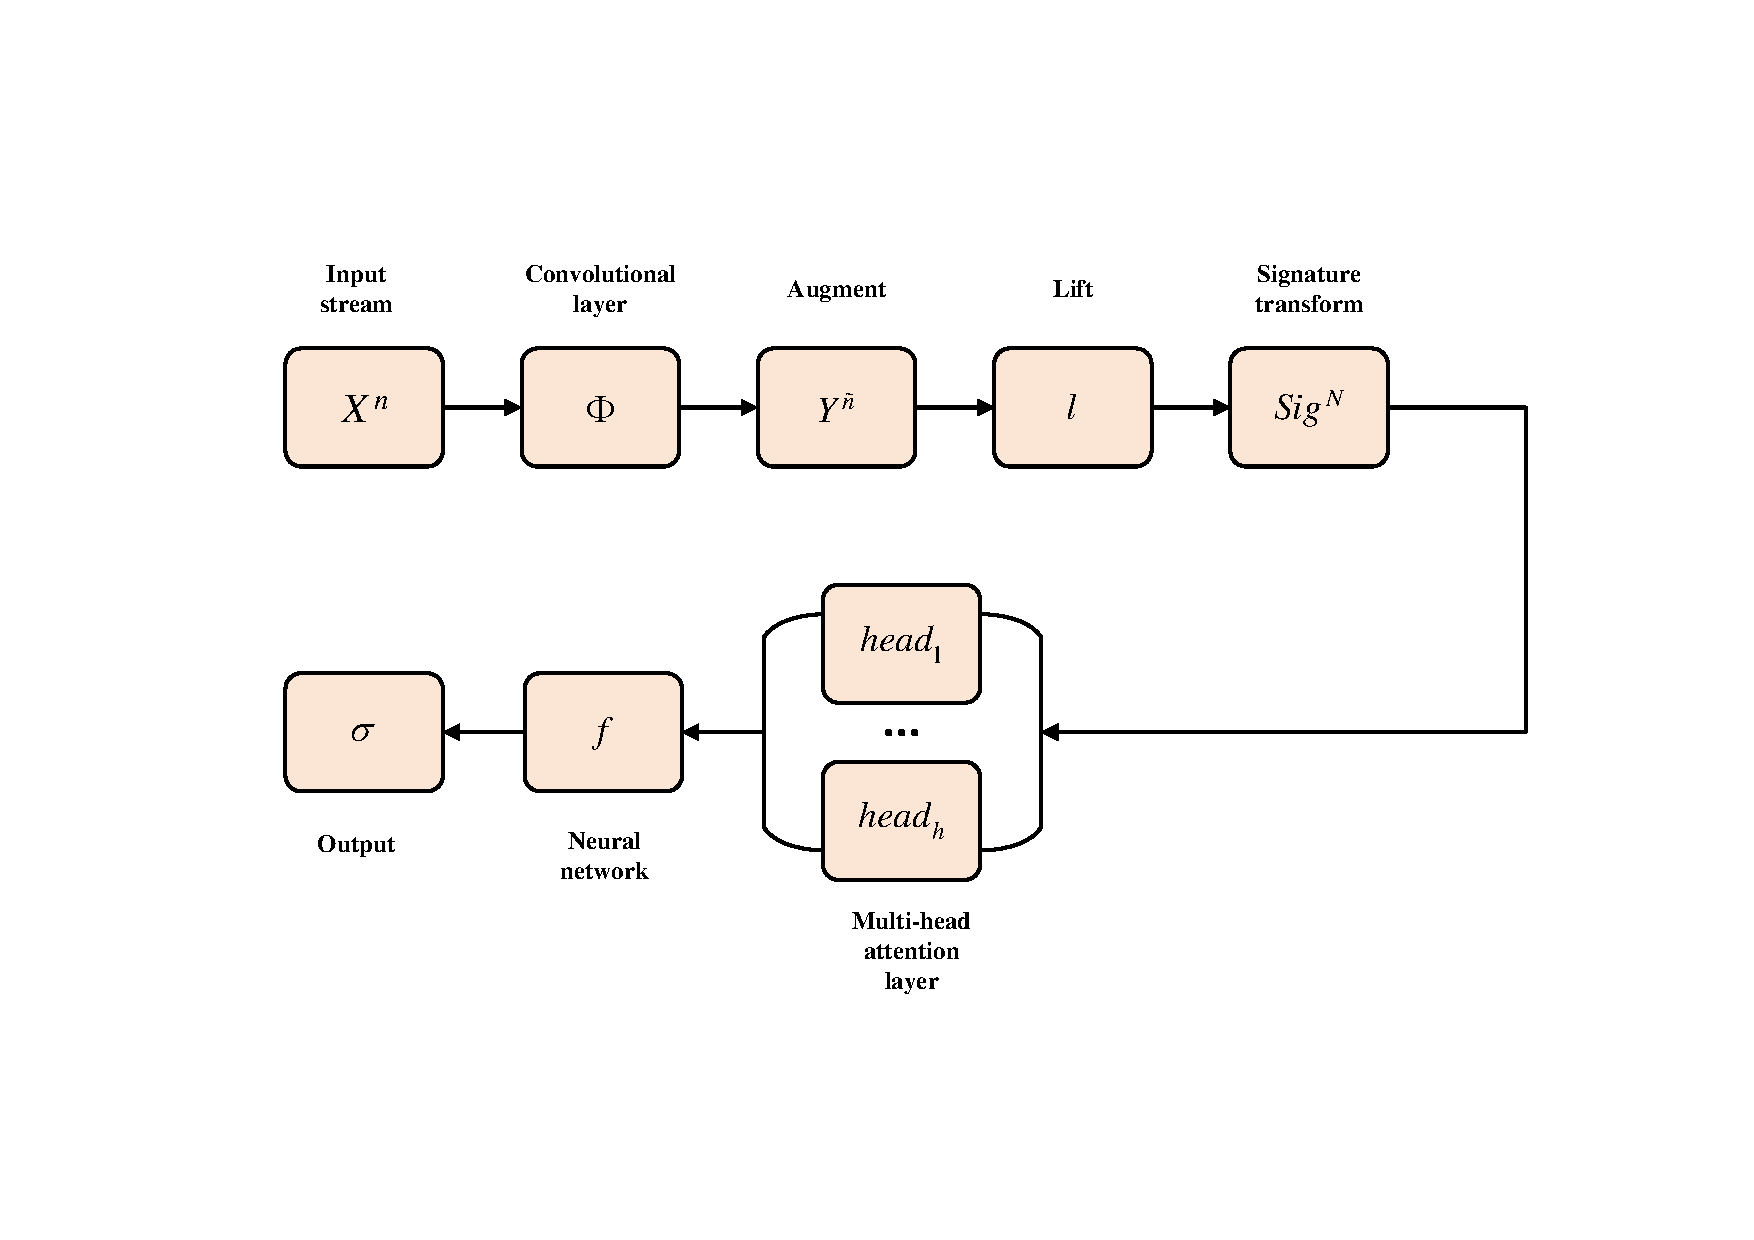
\includegraphics[width=0.8\textwidth]{fig//SigFormer.pdf}
		\caption{Structure of the SigFormer model. }
		\label{fig-structure-sigformer}
	\end{figure}
	
	\section{Numerical experiments}
	\label{sec-experiments}
	Now we will move on to perform some numerical experiments to verify the advantages of this architecture in Section~\ref{sec-methodology} and also to explain why we chose it. Here we choose another two neural network based models for comparison. The first one is a convolutional neural network (CNN) model proposed by \cite{stone_2020} and the corresponding source code is publicly available on \href{https://github.com/henrymstone/rough-calibration-using-CNNS}{Github}\footnote{https://github.com/henrymstone/rough-calibration-using-CNNS}. The other one is a signature-based (DeepSigNet) model proposed by \cite{Lyons_2019_DeepSignature} with  the code on \href{https://github.com/patrick-kidger/Deep-Signature-Transforms}{Github}\footnote{https://github.com/patrick-kidger/Deep-Signature-Transforms}. We also present the specific architecture of these two models  we used in numerical experiments on Appendix~\ref{subapdix-architecture1}. In the following experiments, we will show results of CNN and DeepSigNet model as benchmarks. And we will show the number of model parameters instead of the program runtime to represent the model complexity, in order to avoid the impact of different computational hardware.
	This section is split into two subsections to discuss the single parameter calibration problem and the multiple parameters calibration problem, respectively. 
	
	\subsection{Calibrating the Hurst parameter with rough volatility processes}
	\label{subsec-single-calibration}
	In this section, we perform two examples to verify the advantages of our SigFormer model for single parameter calibration problems and also determine the optimal signature truncation order.
	
	\subsubsection{Implementation details}
	\label{subsubsec-single-implementation}
	In order to generate data sets containing paths with different roughness, we first sample five Hurst parameters $H$ from different probability distributions: the Uniform distribution\footnote{The corresponding set of possible $H$ values is $\{0.06,\,0.12,\,0.27,\,0.35,\,0.45\}$.} on $(0,\,0.5)$ and the $\text{Beta}(1,\,9)$ distribution\footnote{The corresponding set of possible $H$ values is $\{0.04,\,0.08,\,0.11,\,0.16,\,0.21\}$.}. Obviously, paths with $H$ in the Beta distributed set is rougher than those with $H$ in uniformly distributed set. Then we use these different $H$ to simulate fBm, rBergomi and rHeston paths with different number of time steps $\{100,\,200,\,300,\,400,\,500\}$ to generate ten corresponding training/test data sets with the same size as shown in Table~\ref{tab-data-size}.
	\begin{table}[H]
		\caption{Training and test data size.}
		\label{tab-data-size}
		\smallskip
		\centering
		\renewcommand\arraystretch{1.5}
		\begin{tabular}{l c}
			\toprule
			Data set&Number of samples\\
			\hline
			Training set&3000\\
			Test set&1000\\	
			\bottomrule
		\end{tabular}
	\end{table}
	We employ the Cholesky decomposition to simulate fBm and then obtain rBergomi paths with $\eta=1$ and $V_0^{rBergomi}=0.01$; this very well-known simulation technique is recommended because the resulting sample paths have the exact distribution, rather than an approximate distribution, of the normalised log volatility process of the rBergomi volatility process. And we apply the fast algorithm proposed by \cite{ma_2022_fast} with $\kappa_1=0.1,\,\kappa_2=0.03,\,\theta=0.3,\,V_0^{rHeston}=0.01$ to simulate rHeston paths. 
	
	We use adaptive moment estimation (Adam) optimizer to train these models, setting $\textit{batch size}=64$, $\textit{epochs}=100$ and $\textit{leraning rate}=0.0001$ as is fairly standard. We use the mean square error (MSE) as the loss function for training and provide the root mean square error (RMSE) in results as reference.
	
	\subsubsection{Calibrating the Hurst parameter from volatility paths with different lengths}
	\label{subsubsec-single-different}
	In order to validate the necessity of both the convolutional and the fully connected layers in our SigFormer model as well as show our SigFormer is beneficial from multi-head attention, we propose another simple signature-based transformer for comparison, the architecture of this simple SigFormer model is also presented in Appendix~\ref{subapdix-architecture1}. Estimating the Hurst parameter $H$ of a fBm, rBergomi or rHeston path is considered a nontrivial task because of the paths’ non-stationarity and long range dependencies. Therefore paths with more time steps and smaller $H$ (i.e. rougher) are more difficult to calibrate. 
	
	In this example, we train a variety of models that we mentioned before to perform this estimation. That is, to learn the map $(t^n,\,X^n)\mapsto H$, where $t^n$ denotes the time steps and $X^n$ are the corresponding simulated paths. The results are shown in Table~\ref{tab-H-uniform} for $H\sim\text{Uniform}(0,\,0.5)$ and Table~\ref{tab-H-beta} for $H\sim\text{Beta}(1,\,9)$ with the corresponding loss plots shown in Appendix~\ref{subapdix-loss-plots-H}. In order to present the results more clearly, we also plot Table~\ref{tab-H-uniform} and Table~\ref{tab-H-beta} into Figure~\ref{fig-example1-rmse}. 
	From these results, we can easily conclude that the SigFormer model tends to outperform the competing models in three scenarios for single parameter calibration problems: (a) paths with more time steps; (b) rougher paths; (c) paths simulated by more complex volatility models. We attribute this to the self-attention mechanism, which enhances the capacity of the SigFormer model for analyzing information from path signatures, thereby making it outperforming in complex calibration problems. 
	We also observe that the number of parameters i.e. the complexity for the SigFormer model increases with the input length while the Simple SigFormer and DeepSigNet model maintain a constant number of parameters. This feature of the SigFormer model is not directly from introducing the multi-head self-attention layer, but rather through the lifting operation before taking the signature. Furthermore, we need to take the signature multiple times since the lifting operation preserves the stream-like nature of the data, which will increase the input length of the multi-head self-attention layer and subsequently increase the number of model parameters.
	
	\begin{table}[H]
		\caption{Test results for different models with input lengths varying from $100$ to $500$ and $H\sim\text{Uniform}(0,\,0.5)$.}
		\label{tab-H-uniform}
		\smallskip
		\centering
		\renewcommand\arraystretch{1.5}
		\resizebox{\textwidth}{!}{
			\begin{tabular}{l c c c c c}
				\toprule
				\multirow{2}{*}{Models}&\multirow{2}{*}{Input length}&\multicolumn{3}{c}{Test RMSE}&\multirow{2}{*}{$\#$Params}\\
				\cline{3-5}
				&&fBm&rBergomi&rHeston&\\
				\hline
				\multirow{5}{*}{DeepSigNet}
				&100&$1.65\times10^{-2}$&$7.20\times10^{-2}$&$1.39\times10^{-1}$&9261\\
				&200&$1.07\times10^{-2}$&$5.77\times10^{-2}$&$1.21\times10^{-1}$&9261\\
				&300&$1.57\times10^{-2}$&$3.91\times10^{-2}$&$1.40\times10^{-1}$&9261\\
				&400&$1.14\times10^{-2}$&$5.22\times10^{-2}$&$1.19\times10^{-1}$&9261\\
				&500&$2.63\times10^{-2}$&$4.80\times10^{-2}$&$1.34\times10^{-1}$&9261\\
				\hline
				\multirow{5}{*}{CNN}
				&100&$7.53\times10^{-2}$&$4.89\times10^{-2}$&$1.00\times10^{-1}$&255073\\
				&200&$7.80\times10^{-2}$&$5.24\times10^{-2}$&$8.34\times10^{-2}$&320609\\
				&300&$9.23\times10^{-2}$&$4.43\times10^{-2}$&$1.01\times10^{-1}$&386145\\
				&400&$7.92\times10^{-2}$&$3.78\times10^{-2}$&$1.00\times10^{-1}$&435297\\
				&500&$9.05\times10^{-2}$&$5.12\times10^{-2}$&$8.70\times10^{-2}$&500833\\
				\hline
				\multirow{5}{*}{SigFormer}
				&100&$1.34\times10^{-2}$&$5.30\times10^{-2}$&$9.63\times10^{-2}$&126906\\
				&200&$1.38\times10^{-2}$&$4.77\times10^{-2}$&$7.34\times10^{-2}$&176506\\
				&300&$1.28\times10^{-2}$&$4.12\times10^{-2}$&$4.45\times10^{-2}$&226106\\
				&400&$1.42\times10^{-2}$&$4.00\times10^{-2}$&$4.29\times10^{-2}$&275706\\
				&500&$1.27\times10^{-2}$&$3.69\times10^{-2}$&$3.77\times10^{-2}$&325306\\
				\hline
				\multirow{5}{*}{Simple SigFormer}
				&100&$6.83\times10^{-2}$&$1.47\times10^{-1}$&$1.44\times10^{-1}$&6666\\
				&200&$7.03\times10^{-2}$&$1.42\times10^{-1}$&$1.43\times10^{-1}$&6666\\
				&300&$6.93\times10^{-2}$&$1.44\times10^{-1}$&$1.46\times10^{-1}$&6666\\
				&400&$6.69\times10^{-2}$&$1.42\times10^{-1}$&$1.41\times10^{-1}$&6666\\
				&500&$6.32\times10^{-2}$&$1.42\times10^{-1}$&$1.45\times10^{-1}$&6666\\
				\bottomrule	
			\end{tabular}
		}
	\end{table}

	\begin{table}[H]
		\caption{Test results for different models with input lengths varying from $100$ to $500$ and $H\sim\text{Beta}(1,\,9)$.}
		\label{tab-H-beta}
		\smallskip
		\centering
		\renewcommand\arraystretch{1.5}
		\resizebox{\textwidth}{!}{
			\begin{tabular}{l c c c c c}
				\toprule
				\multirow{2}{*}{Models}&\multirow{2}{*}{Input length}&\multicolumn{3}{c}{Test RMSE}&\multirow{2}{*}{$\#$Params}\\
				\cline{3-5}
				&&fBm&rBergomi&rHeston&\\
				\hline
				\multirow{5}{*}{DeepSigNet}
				&100&$1.31\times10^{-2}$&$5.55\times10^{-2}$&$6.04\times10^{-2}$&9261\\
				&200&$1.14\times10^{-2}$&$4.68\times10^{-2}$&$5.83\times10^{-2}$&9261\\
				&300&$1.58\times10^{-2}$&$4.77\times10^{-2}$&$5.82\times10^{-2}$&9261\\
				&400&$2.44\times10^{-2}$&$4.23\times10^{-2}$&$5.84\times10^{-2}$&9261\\
				&500&$2.24\times10^{-2}$&$3.83\times10^{-2}$&$5.83\times10^{-2}$&9261\\
				\hline
				\multirow{5}{*}{CNN}
				&100&$1.39\times10^{-1}$&$5.68\times10^{-2}$&$8.57\times10^{-2}$&255073\\
				&200&$9.24\times10^{-2}$&$5.24\times10^{-2}$&$8.44\times10^{-2}$&320609\\
				&300&$9.39\times10^{-2}$&$6.30\times10^{-2}$&$8.78\times10^{-2}$&386145\\
				&400&$8.87\times10^{-2}$&$5.23\times10^{-2}$&$7.86\times10^{-2}$&435297\\
				&500&$9.18\times10^{-2}$&$5.32\times10^{-2}$&$7.60\times10^{-2}$&500833\\
				\hline
				\multirow{5}{*}{SigFormer}
				&100&$1.38\times10^{-2}$&$3.76\times10^{-2}$&$5.83\times10^{-2}$&126906\\
				&200&$1.81\times10^{-2}$&$3.68\times10^{-2}$&$5.17\times10^{-2}$&176506\\
				&300&$1.81\times10^{-2}$&$3.63\times10^{-2}$&$4.77\times10^{-2}$&226106\\
				&400&$1.85\times10^{-2}$&$2.63\times10^{-2}$&$1.37\times10^{-2}$&275706\\
				&500&$1.34\times10^{-2}$&$2.54\times10^{-2}$&$1.44\times10^{-2}$&325306\\
				\hline
				\multirow{5}{*}{Simple SigFormer}
				&100&$3.64\times10^{-2}$&$5.95\times10^{-2}$&$6.08\times10^{-2}$&6666\\
				&200&$3.51\times10^{-2}$&$6.08\times10^{-2}$&$5.88\times10^{-2}$&6666\\
				&300&$3.70\times10^{-2}$&$5.99\times10^{-2}$&$5.87\times10^{-2}$&6666\\
				&400&$3.62\times10^{-2}$&$6.00\times10^{-2}$&$5.99\times10^{-2}$&6666\\
				&500&$4.05\times10^{-2}$&$5.90\times10^{-2}$&$5.96\times10^{-2}$&6666\\
				\bottomrule	
			\end{tabular}
		}
	\end{table}
	
	\begin{figure}[H]
		\centering
		\resizebox{0.9\textwidth}{!}{
			\subfigure[$H\sim\text{Uniform}(0,0.5)$]{
				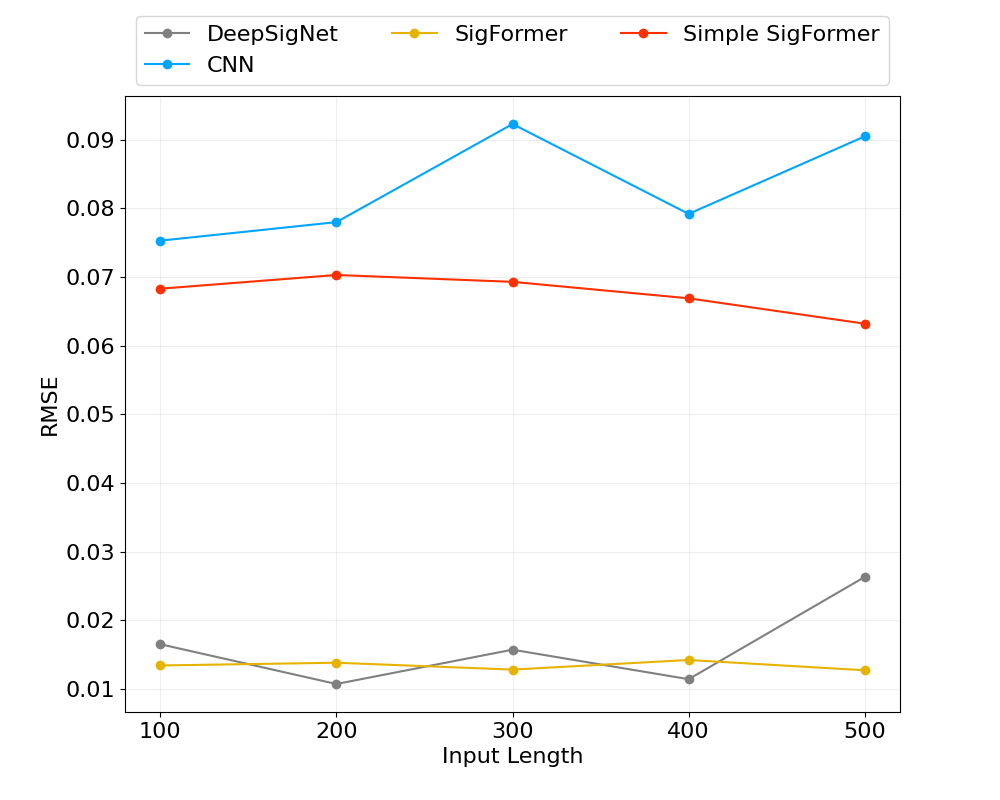
\includegraphics[width=0.32\textwidth]{fig//example1_Huniform_fBm.png}
				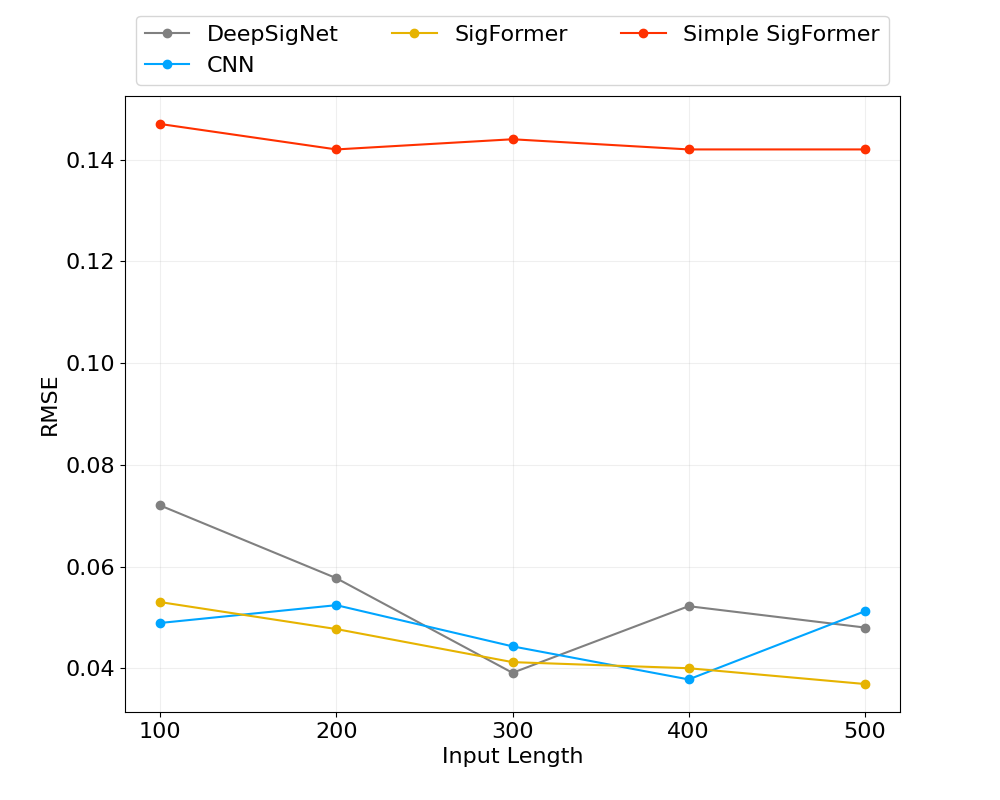
\includegraphics[width=0.32\textwidth]{fig//example1_Huniform_rBergomi.png}
				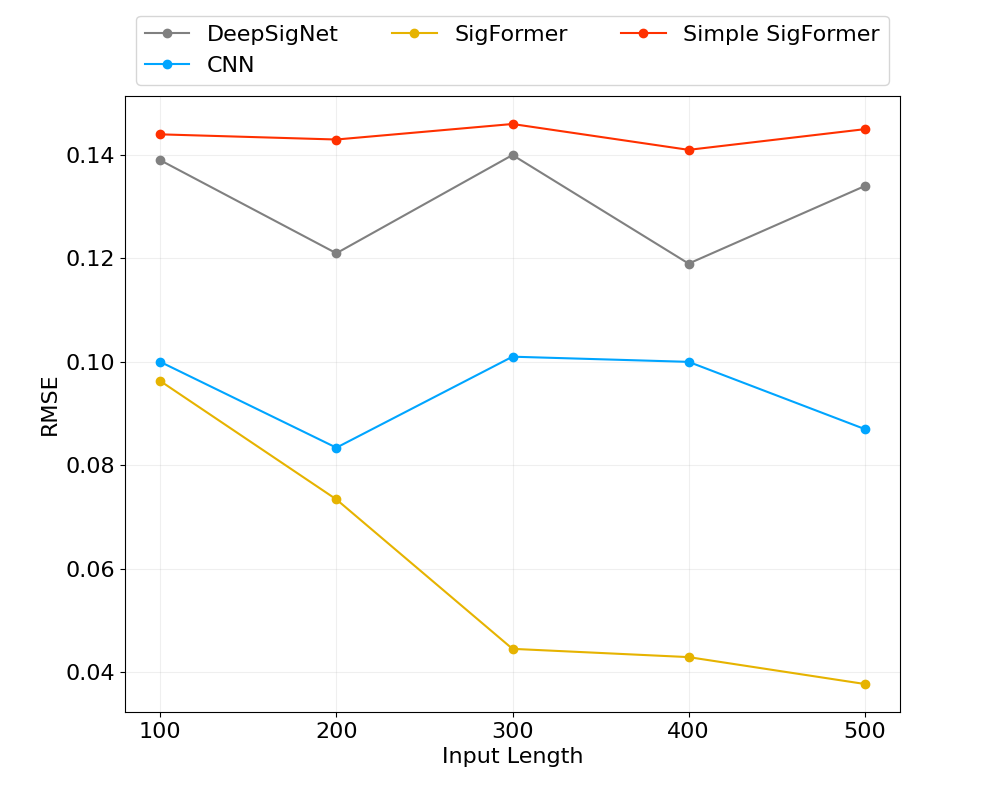
\includegraphics[width=0.32\textwidth]{fig//example1_Huniform_rHeston.png}}
		}
		\resizebox{0.9\textwidth}{!}{
			\subfigure[$H\sim\text{Beta}(1,\,9)$]{
				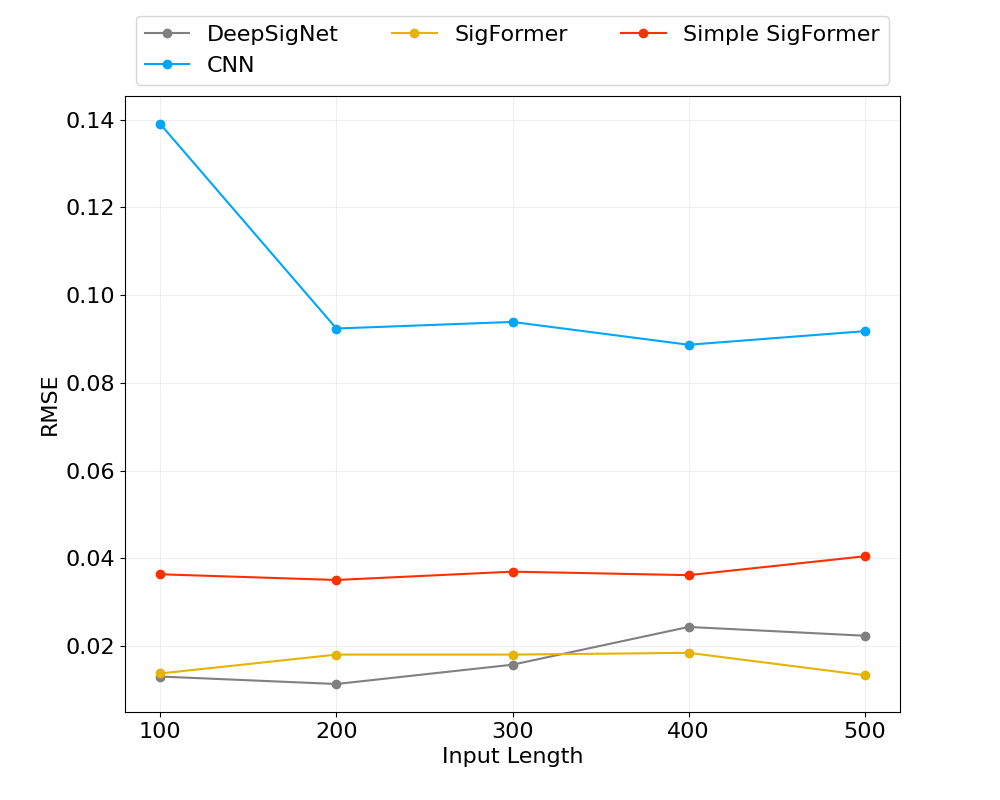
\includegraphics[width=0.32\textwidth]{fig//example1_Hbeta_fBm.png}
				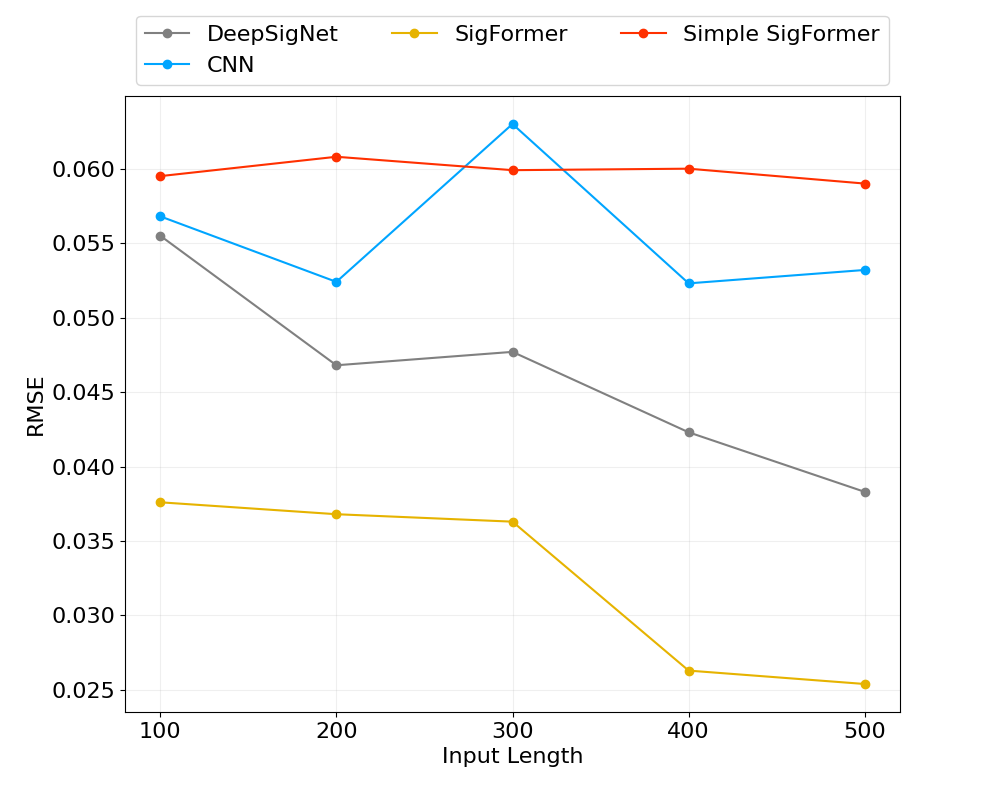
\includegraphics[width=0.32\textwidth]{fig//example1_Hbeta_rBergomi.png}
				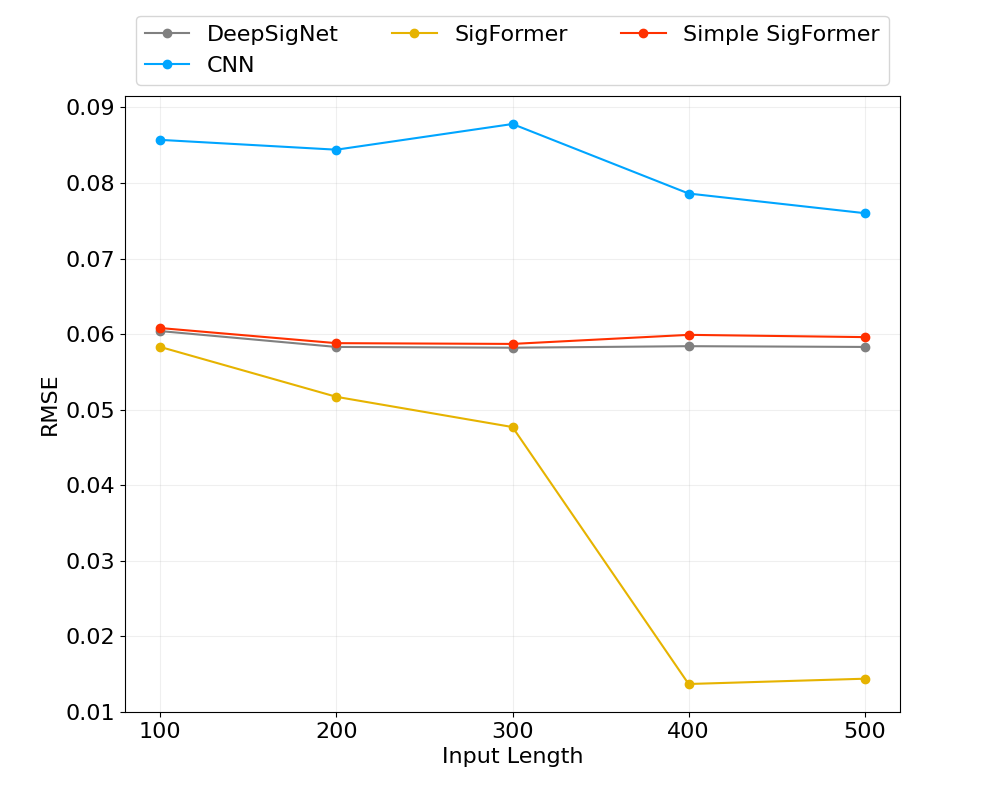
\includegraphics[width=0.32\textwidth]{fig//example1_Hbeta_rHeston.png}}
		}
		\caption{RMSE of calibrating $H$  for different volatility models (Left: fBms; Middle: rBergomi volatility processes; Right: rHeston volatility processes) over input lengths vary from $100$ to $500$. }
		\label{fig-example1-rmse}
	\end{figure}
	
	\subsubsection{Calibrating the Hurst parameter from volatility paths with different signature truncation orders}
	\label{subsubsec-single-truncation}
	From the previous example, we have verified the advantages of our SigFormer model in single parameter calibration problems. Following the analysis at the beginning of Section~\ref{subsec-single-calibration}, we aim to explore the effects of varying signature truncation orders on our SigFormer model next. 
	In this example, we will only use the paths with $H\sim\text{Beta}(1,\,9)$ and $100$ time steps for simplicity. And we modify the signature truncation order to vary from $\{1,\,2,\,3,\,4,\,5\}$ while keeping other settings the same as Section~\ref{subsubsec-single-implementation}.
	
	The results are shown in Table~\ref{tab-H-truncation} with the corresponding loss plots shown in Appendix~\ref{subapdix-loss-plots-truncation}. In order to present the results more clearly, we also plot Table~\ref{tab-H-truncation} into Figure~\ref{fig-example2-truncation}. It is evident that the optimal signature truncation orders for our SigFormer model vary across different volatility models; specifically, the order is $2$ for fBm, $4$ for rBergomi, and $5$ for rHeston. We also notice that the signature truncation order is correlated with the model complexity, thus we select the truncation order equal to $3$ in our SigFormer model for the balance between performance and complexity.
	
	\begin{table}[H]
		\caption{Test results for different models with the signature truncation order varying from $1$ to $5$. Here $H\sim\text{Beta}(1,\,9)$ and the input lengths equal to $100$.}
		\label{tab-H-truncation}
		\smallskip
		\centering
		\renewcommand\arraystretch{1.5}
		\resizebox{\textwidth}{!}{
			\begin{tabular}{l c c c c c}
				\toprule
				&\multicolumn{2}{c}{Test RMSE} & & &\\
				\cline{2-4}
				& fBm & rBergomi & rHeston & $\#$Params &Truncation order\\
				\hline
				DeepSigNet &$4.37\times10^{-2}$&$5.95\times10^{-2}$&$6.08\times10^{-2}$&4461&\multirow{3}{*}{1}\\
				SigFormer &$2.60\times10^{-2}$&$5.95\times10^{-2}$&$6.07\times10^{-2}$&6006&\\
				Simple SigFormer &$5.91\times10^{-2}$&$5.95\times10^{-2}$&$6.08\times10^{-2}$&1086&\\
				\hline
				DeepSigNet &$8.64\times10^{-3}$&$5.60\times10^{-2}$&$6.05\times10^{-2}$&5261&\multirow{3}{*}{2}\\
				SigFormer &$8.60\times10^{-3}$&$5.05\times10^{-2}$&$6.01\times10^{-2}$&16781&\\
				Simple SigFormer &$5.67\times10^{-2}$&$5.95\times10^{-2}$&$6.08\times10^{-2}$&2946&\\
				\hline
				DeepSigNet &$1.59\times10^{-2}$&$5.02\times10^{-2}$&$6.03\times10^{-2}$&9261&\multirow{3}{*}{3}\\
				SigFormer &$1.37\times10^{-2}$&$4.26\times10^{-2}$&$5.75\times10^{-2}$&126906&\\
				Simple SigFormer &$4.00\times10^{-2}$&$5.95\times10^{-2}$&$6.08\times10^{-2}$&6666&\\
				\hline
				DeepSigNet &$3.23\times10^{-2}$&$5.25\times10^{-2}$&$6.01\times10^{-2}$&29261&\multirow{3}{*}{4}\\
				SigFormer &$2.11\times10^{-2}$&$3.61\times10^{-2}$&$5.34\times10^{-2}$&2083781&\\
				Simple SigFormer &$3.09\times10^{-2}$&$5.95\times10^{-2}$&$6.08\times10^{-2}$&14106&\\
				\hline
				DeepSigNet &$5.74\times10^{-2}$&$4.85\times10^{-2}$&$6.02\times10^{-2}$&129261&\multirow{3}{*}{5}\\
				SigFormer &$8.25\times10^{-2}$&$3.93\times10^{-2}$&$5.24\times10^{-2}$&47024406&\\
				Simple SigFormer &$2.53\times10^{-2}$&$5.95\times10^{-2}$&$6.08\times10^{-2}$&28986&\\
				\bottomrule
		\end{tabular}
	}
	\end{table}
	
	\begin{figure}[H]
		\centering
		\label{fig-example2-truncation}
		
\includegraphics[width=0.32\textwidth]{fig//example2_fBm.png}
		
\includegraphics[width=0.32\textwidth]{fig//example2_rBergomi.png}
		
\includegraphics[width=0.32\textwidth]{fig//example2_rHeston.png}
		\caption{RMSE of calibrating $H$  for different volatility models (Left: fBms; Middle: rBergomi volatility processes; Right: rHeston volatility processes) over signature truncation order varying from $1$ to $5$.}
	\end{figure}


	\subsection{Calibrating multiple parameters with rough volatility processes}
	\label{subsec-multiple-calibration}
	In previous examples, we have observed that the SigFormer model tends to outperform competing models in more complex calibration problems, such as those involving paths simulated by advanced volatility models and more time steps. Therefore, it is natural to consider applying the SigFormer model in multiple parameters calibration problems. Furthermore, we also want to simplify the SigFormer model without losing too much accuracy since the complexity of the SigFormer model will increase with the input length as shown in Section~\ref{subsubsec-single-different}.
	
	In this section, we will perform two examples: the first example will verify the advantages of our SigFormer model for multiple parameters calibration problems and the second example will show how to reduce the complexity of the SigFormer model with minimal loss of accuracy. 
	
	\subsubsection{Implementation details}
	\label{subsubsec-multiple-implementation}
	In order to generate the data sets for multiple parameters calibration problems, we first sample different $\eta,\kappa_1,\,\kappa_2,\,\theta$ from the distribution shown in Table~\ref{tab-multiple-distribution}. Then we simulate rBergomi and rHeston paths with these parameters, as well as $H\sim\text{Beta}(1,\,9)$, from Section~\ref{subsubsec-single-implementation} to generate four corresponding training/test data sets with the same size as shown in Table~\ref{tab-data-size} and all paths are simulated $100$ steps. The first data set consists of rBergomi paths with different $\eta$ and $H$. The second data set consists of rHeston paths with different $\kappa_2$ and $H$ while keeping $\kappa_1=0.1$ and $\theta=0.3$. The third data set consists of rHeston paths with different $\kappa_1,\,\kappa_2$ and $H$ while keeping $\theta=0.3$. The fourth data set consists of rHeston paths with different $\kappa_1,\,\kappa_2,\,\theta$ and $H$. All other settings are kept the same as Section~\ref{subsubsec-single-implementation}.
	\begin{table}[H]
		\caption{Distributions for sampling parameters.}
		\label{tab-multiple-distribution}
		\smallskip
		\centering
		\renewcommand\arraystretch{1.5}
		\begin{tabular}{l c c}
			\toprule
			Parameters&Distributions&Values\\
			\hline
			$\eta$&$\text{Uniform}(0,\,3)$&$\{0.41,\,1.04,\,1.56,\,2.40,\,2.73\}$\\
			$\kappa_1$&$\text{Uniform}(0,\,5)$&$\{0.25,\,1.24,\,2.83,\,3.02,\,4.81\}$\\
			$\kappa_2$&$\text{Uniform}(0,\,3)$&$\{0.13,\,0.79,\,1.58,\,2.23,\,2.94\}$\\
			$\theta$&$\text{Uniform}(0,\,0.5)$&$\{0.05,\,0.14,\,0.21,\,0.30,\,0.42\}$\\
			\bottomrule
		\end{tabular}
	\end{table}
	
	\subsubsection{Multiple parameters calibration}
	\label{subsubsec-multiple-attention}
	We begin this section by calibrating two parameters simultaneously: $H,\,\eta$ of rBergomi volatility processes and $H,\,\kappa_2$ of rHeston volatility processes. The results are shown in Table~\ref{tab-multiple-two} with the corresponding loss plots shown in Appendix~\ref{subapdix-loss-plots-multiple}.
	
	\begin{table}[H]
		\caption{Test results for two parameters calibration with $H\sim\text{Beta}(1,\,9)$, $\eta\sim\text{Uniform}(0,\,3)$ and $\kappa_2\sim\text{Uniform}(0,\,3)$.}
		\label{tab-multiple-two}
		\smallskip
		\centering
		\renewcommand\arraystretch{1.5}
		\begin{tabular}{l c c c}
				\toprule
				\multirow{2}{*}{Models}&\multicolumn{2}{c}{RMSE}&\multirow{2}{*}{$\#$Params}\\
				\cline{2-3}
				&rBergomi&rHeston&\\
				\hline
				CNN&0.729&0.786&255202\\
				\hline
				DeepSigNet&0.728&0.785&9294\\
				\hline
				SigFormer&0.315&0.422&126939\\
				\hline
				Simple SigFormer&0.592&0.708&6822\\
				\bottomrule
		\end{tabular}
	\end{table}
	
	Furthermore, we also perform three and four parameters calibrations for rHeston volatility processes. The results are shown in Table~\ref{tab-multiple-threefour} with the corresponding loss plots shown in Appendix~\ref{subapdix-loss-plots-multiple}. In these multiple calibration problems, we observe that the Simple SigFormer model achieves the same accuracy as the baseline models while requiring fewer model parameters. As for the SigFormer model, it outperforms all other models while requiring more model parameters. These results further demonstrate the advantages of combining self-attention mechanism with the signature transform for calibrating complex rough paths.
	
	\begin{table}[H]
		\caption{Test results for three and four parameters calibration with $H\sim\text{Beta}(1,\,9)$, $\kappa_1\sim\text{Uniform}(0,\,5)$ and $\kappa_2\sim\text{Uniform}(0,\,3)$.}
		\label{tab-multiple-threefour}
		\smallskip
		\centering
		\renewcommand\arraystretch{1.5}
		\begin{tabular}{l c c c}
			\toprule
			Models&&RMSE of rHeston&$\#$Params\\
			\hline
			\multirow{2}{*}{CNN}&$\theta=0.3$&1.400&255331\\
			&$\theta\sim\text{U}(0,\,0.5)$&1.180&255460\\
			\hline
			\multirow{2}{*}{DeepSigNet}&$\theta=0.3$&1.401&9327\\
			&$\theta\sim\text{U}(0,\,0.5)$&1.190&9360\\
			\hline
			\multirow{2}{*}{SigFormer}&$\theta=0.3$&0.700&126972\\
			&$\theta\sim\text{U}(0,\,0.5)$&0.750&127005\\
			\hline
			\multirow{2}{*}{Simple SigFormer}&$\theta=0.3$&1.063&6978\\
			&$\theta\sim\text{U}(0,\,0.5)$&0.926&7134\\
			\bottomrule
		\end{tabular}
	\end{table}
	
	\subsubsection{Lower the complexity for the SigFormer model}
	\label{subsubsec-multiple-complexity}
	From the previous example, we have observed that the Simple SigFormer model can achieve great accuracy with fewer model parameters compared to baseline models, while the SigFormer model outperformed all other models, but it requires a more complex structure. One of the differences between the SigFormer model and the Simple SigFormer model is that the former performs the lifting operation before taking the signature, while the latter does not.
	As mentioned in Section~\ref{subsubsec-single-different}, the lifting operation adds complexity to the SigFormer model; therefore, modifying the stride of the lifting operation could potentially reduce this complexity with minimal loss of accuracy. In this example, we will only use the paths with $H\sim\text{Beta}(1,\,9)$, $\kappa_1\sim\text{Uniform}(0,\,5)$, $\kappa_2\sim\text{Uniform}(0,\,3)$, $\theta\sim\text{Uniform}(0,\,0.5)$ and $100$ time steps. And we modify the stride of the lifting operation to vary from $\{1,\,5,\,10,\,50\}$ while keeping other settings the same as Section~\ref{subsubsec-multiple-attention}.
	
	The results are shown in Table~\ref{tab-multiple-complexity} with the corresponding loss plots shown in Appendix~\ref{subapdix-loss-plots-complexity}. We observe that an increase in the stride can significantly reduce the number of required model parameters without substantially compromising accuracy.
	\begin{table}[H]
		\caption{Test results for the SigFormer model with the stride varying from $1$ to $50$. Here $H\sim\text{Beta}(1,\,9)$, $\kappa_1\sim\text{Uniform}(0,\,5)$, $\kappa_2\sim\text{Uniform}(0,\,3)$, $\theta\sim\text{Uniform}(0,\,0.5)$ and the input lengths equal to $100$. }
		\label{tab-multiple-complexity}
		\smallskip
		\centering
		\renewcommand\arraystretch{1.5}
		\begin{tabular}{l c c c}
			\toprule
			Models&Stride&RMSE of rHeston&$\#$Params\\
			\hline
			\multirow{4}{*}{SigFormer}&1&0.745&573405\\
			&5&0.754&176605\\
			&10&0.761&127005\\
			&50&0.774&87325\\
			\bottomrule
		\end{tabular}
	\end{table}
	
	\section{Conclusion}
	\label{sec-conclusion}
	There is a solid theoretical ground for using the signature transform as a tool to calibrate the streams of data. Meanwhile transformers have enjoyed great empirical success in handling sequential data. It is thus natural to combine them together to calibrate volatility processes; in this paper we have constructed a SigFormer model to present how to do this, and also have provided examples to explore the performance of the SigFormer model in different calibration problems.
	
	There are two main contributions in this paper. First, we give the way to combine the signature transform with the self-attention mechanism. Second, we present how to specify the details of the SigFormer model as well as how to simplify it without substantially compromising accuracy.
	
	%References
	\begin{thebibliography}{10}
%		\bibitem[\protect\citeauthoryear{Bayer and Breneis}{2023}]{Bayer_2023_simulation}
%		Bayer, C., and Breneis, S. (2023). Efficient option pricing in the rough Heston model using weak simulation schemes. arXiv preprint arXiv:2310.04146.

		\bibitem[\protect\citeauthoryear{Hambly and Lyons}{2010}]{Lyons_2010_uniqueness}
		Hambly, B., and Lyons, T. (2010). Uniqueness for the signature of a path of bounded variation and the reduced path group. Annals of Mathematics, 109-167.
		
		\bibitem[\protect\citeauthoryear{Horvath, Muguruza and Tomas}{2021}]{horvath2021deep}
		Horvath, B., Muguruza, A. and Tomas, M. (2021). Deep learning volatility: a deep neural network perspective on pricing and calibration in (rough) volatility models. Quantitative Finance, 21, 11--27.
		
		\bibitem[\protect\citeauthoryear{Kidger, Bonnier, Perez Arribas, Salvi and Lyons}{2019}]{Lyons_2019_DeepSignature}
		Kidger, P., Bonnier, P., Perez Arribas, I., Salvi, C., and Lyons, T. (2019). Deep signature transforms. Advances in Neural Information Processing Systems, 32.
		
		\bibitem[\protect\citeauthoryear{Lyons}{1998}]{Lyons_1998_decay}
		Lyons, T. J. (1998). Differential equations driven by rough signals. Revista Matemática Iberoamericana, 14(2), 215-310.
		
		\bibitem[\protect\citeauthoryear{Ma and Wu}{2022}]{ma_2022_fast}
		Ma, J. and Wu, H. (2022). A fast algorithm for simulation of rough volatility models. Quantitative Finance, 22, 447--462.
		
		\bibitem[\protect\citeauthoryear{Ma, J., Wu, X., and Wu, H.}{2023}]{ma2023rough}
		Ma, J., Wu, X., and Wu, H. A neural network rough volatility model. https://rgdoi.net/10.13140/RG.2.2.30650.98249
		
		\bibitem[\protect\citeauthoryear{Mandelbrot and Van Ness}{1968}]{mandelbrot_1968_fbm}
		Mandelbrot, B. B., and Van Ness, J. W. (1968). Fractional Brownian motions, fractional noises and applications. SIAM review, 10(4), 422-437.
		
		\bibitem[\protect\citeauthoryear{Rosenbaum and Zhang}{2021}]{rosenbaum2021deep}
		Rosenbaum, M. and Zhang, J.F. (2022). Deep calibration of the quadratic rough Heston model.
		https://doi.org/10.48550/arXiv.2102.01962
		
		\bibitem[\protect\citeauthoryear{Stone}{2020}]{stone_2020}
		Stone, H. (2020). Calibrating rough volatility models: a convolutional neural network approach. Quantitative Finance, 20(3), 379-392.
		
		\bibitem[\protect\citeauthoryear{Tong}{2023}]{tong_2023}
		Tong, A., Nguyen-Tang, T., Lee, D., Tran, T. M., and Choi, J. (2023, November). SigFormer: Signature Transformers for Deep Hedging. In Proceedings of the Fourth ACM International Conference on AI in Finance (pp. 124-132).
		
		\bibitem[\protect\citeauthoryear{Vaswani, A., Shazeer, N., Parmar, N., Uszkoreit, J., Jones, L., Gomez, A. N., Kaiser L. and Polosukhin, I.}{2017}]{vaswani_2017}
		Vaswani, A., Shazeer, N., Parmar, N., Uszkoreit, J., Jones, L., Gomez, A. N., Kaiser L. and Polosukhin, I. (2017). Attention is all you need. Advances in neural information processing systems, 30.
		
		\bibitem[\protect\citeauthoryear{Wang and Hong}{2021}]{wang2021NSDE}
		Wang, S.D. and Hong, L.J. (2021). Option pricing by neural stochastic differential equations: a simulation-optimization approach. 2021 Winter Simulation Conference (WSC), 1--11. doi: 10.1109/WSC52266.2021.9715493
		
		
		
	\end{thebibliography}
	
	\appendix
	\section{Architecture of different models}
	\subsection{Architecture of CNN and DeepSigNet model}
	\label{subapdix-architecture1}
	Here we clarify the specific architecture of CNN and DeepSigNet model as below
	\begin{itemize}
		\item The architecture of CNN model:
		\begin{itemize}
			\item[-] a convolutional layer with 32 channels and kernel size 20;
			\item[-] the leaky ReLu transform with negative slope 0.1;
			\item[-] a max pooling layer with size 3;
			\item[-] a dropout layer with rate 0.25;			
			\item[-] a convolutional layer with 64 channels and kernel size 20;
			\item[-] the leaky ReLu transform with negative slope 0.3;
			\item[-] a max pooling layer with size 3;
			\item[-] a dropout layer with rate 0.25;
			\item[-] a convolutional layer with 128 channels and kernel size 20;
			\item[-] the leaky ReLu transform with negative slope 0.1;
			\item[-] a max pooling layer with size 3;
			\item[-] a dropout layer with rate 0.4;
			\item[-] a dense layer with 128 units;
			\item[-] the leaky ReLu transform with negative slope 0.1;
			\item[-] a dropout layer with rate 0.3;
			\item[-] a dense layer with 1 units;
			\item[-] a non-linear transform with sigmoid function.			
		\end{itemize}
		\item The architecture of DeepSigNet model:
		\begin{itemize}
			\item[-] a convolutional layer with 3 channels and kernel size 3;
			\item[-] augmented with time and original values;
			\item[-] taking the signature transform with truncation order $N=3$;
			\item[-] a fully connected feedforward neural network with 5 hidden layers, each of size 32 and ReLU activation;
			\item[-] a non-linear transform with sigmoid function.
		\end{itemize}
		\item The architecture of simple SigFormer model:
		\begin{itemize}
			\item[-] augmented with time;
			\item[-] taking the signature transform with truncation order $N=3$;
			\item[-] a single-head self-attention layer;
			\item[-] a non-linear transform with sigmoid function.
		\end{itemize}
	\end{itemize}

	
	\section{Loss plots}
	\label{apdix-loss-plots}
	\subsection{Loss plots for different models with input lengths varying from $100$ to $500$}
	\label{subapdix-loss-plots-H}
	\begin{figure}[H]
		\centering
		\resizebox{0.9\textwidth}{!}{
		\subfigure[$H\sim\text{Uniform}(0,0.5)$]{
			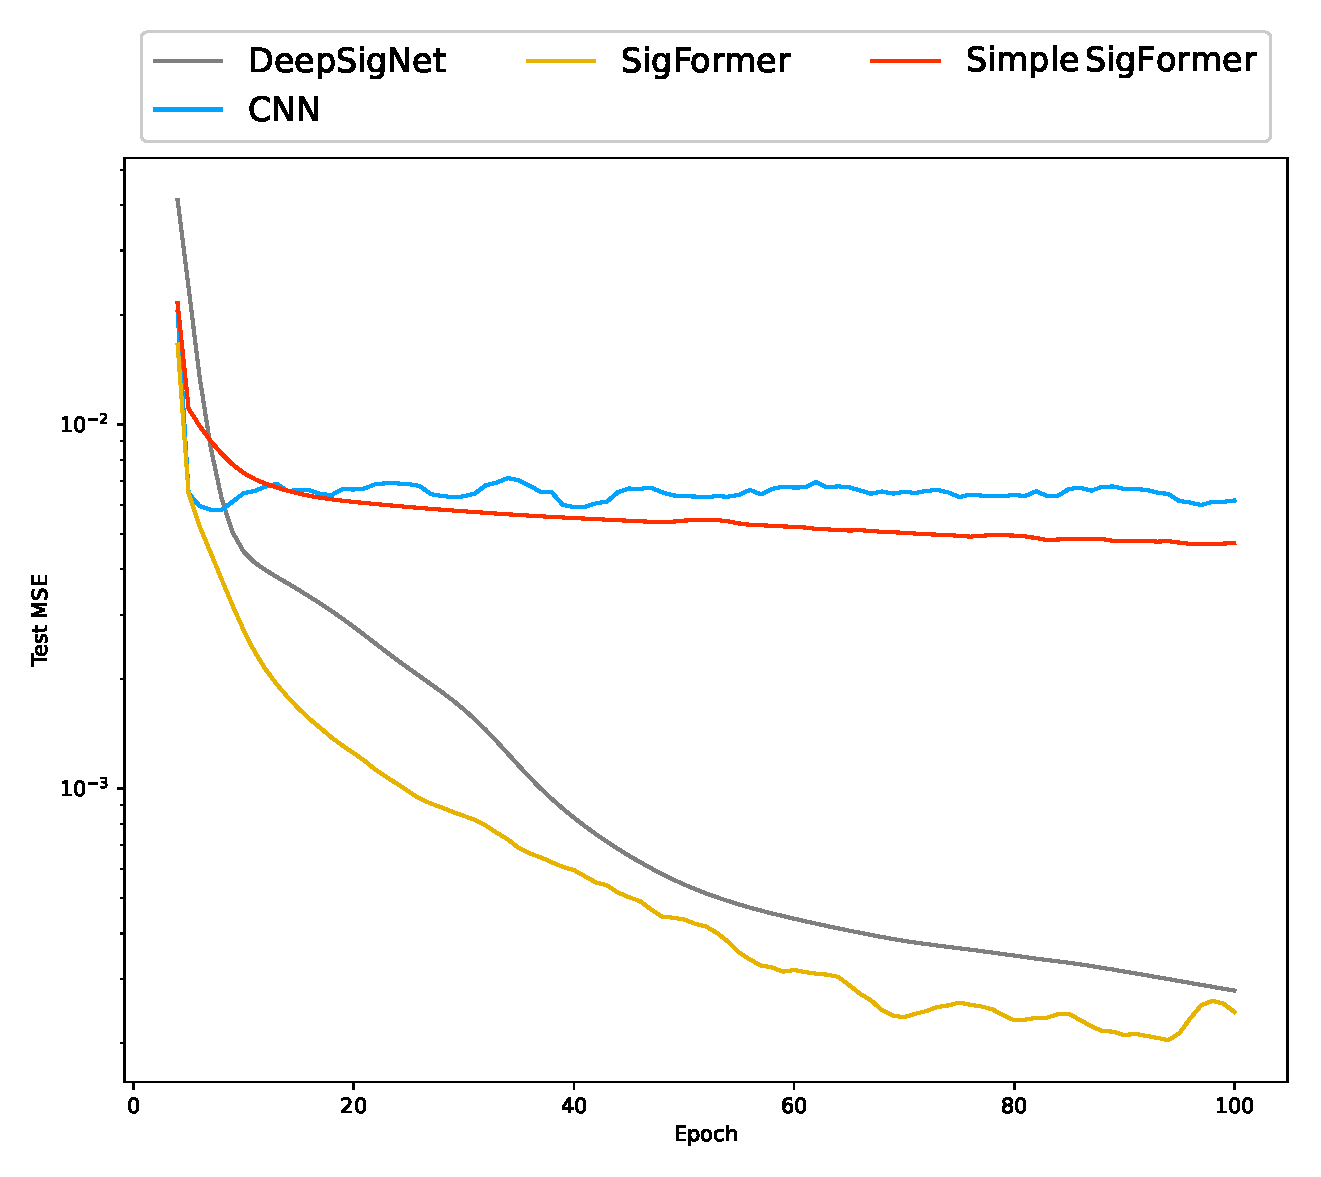
\includegraphics[width=0.32\textwidth]{fig//fBm_grid=100_Huniform.eps}
			
\includegraphics[width=0.32\textwidth]{fig//rBergomi_grid=100_Huniform_eta=1_v0=0.01.eps}
			
\includegraphics[width=0.32\textwidth]{fig//rHeston_grid=100_Huniform_kappa1=0.1_kappa2=0.03_theta=0.3_v0=0.01.eps}}
		}
		\resizebox{0.9\textwidth}{!}{
		\subfigure[$H\sim\text{Beta}(1,\,9)$]{
			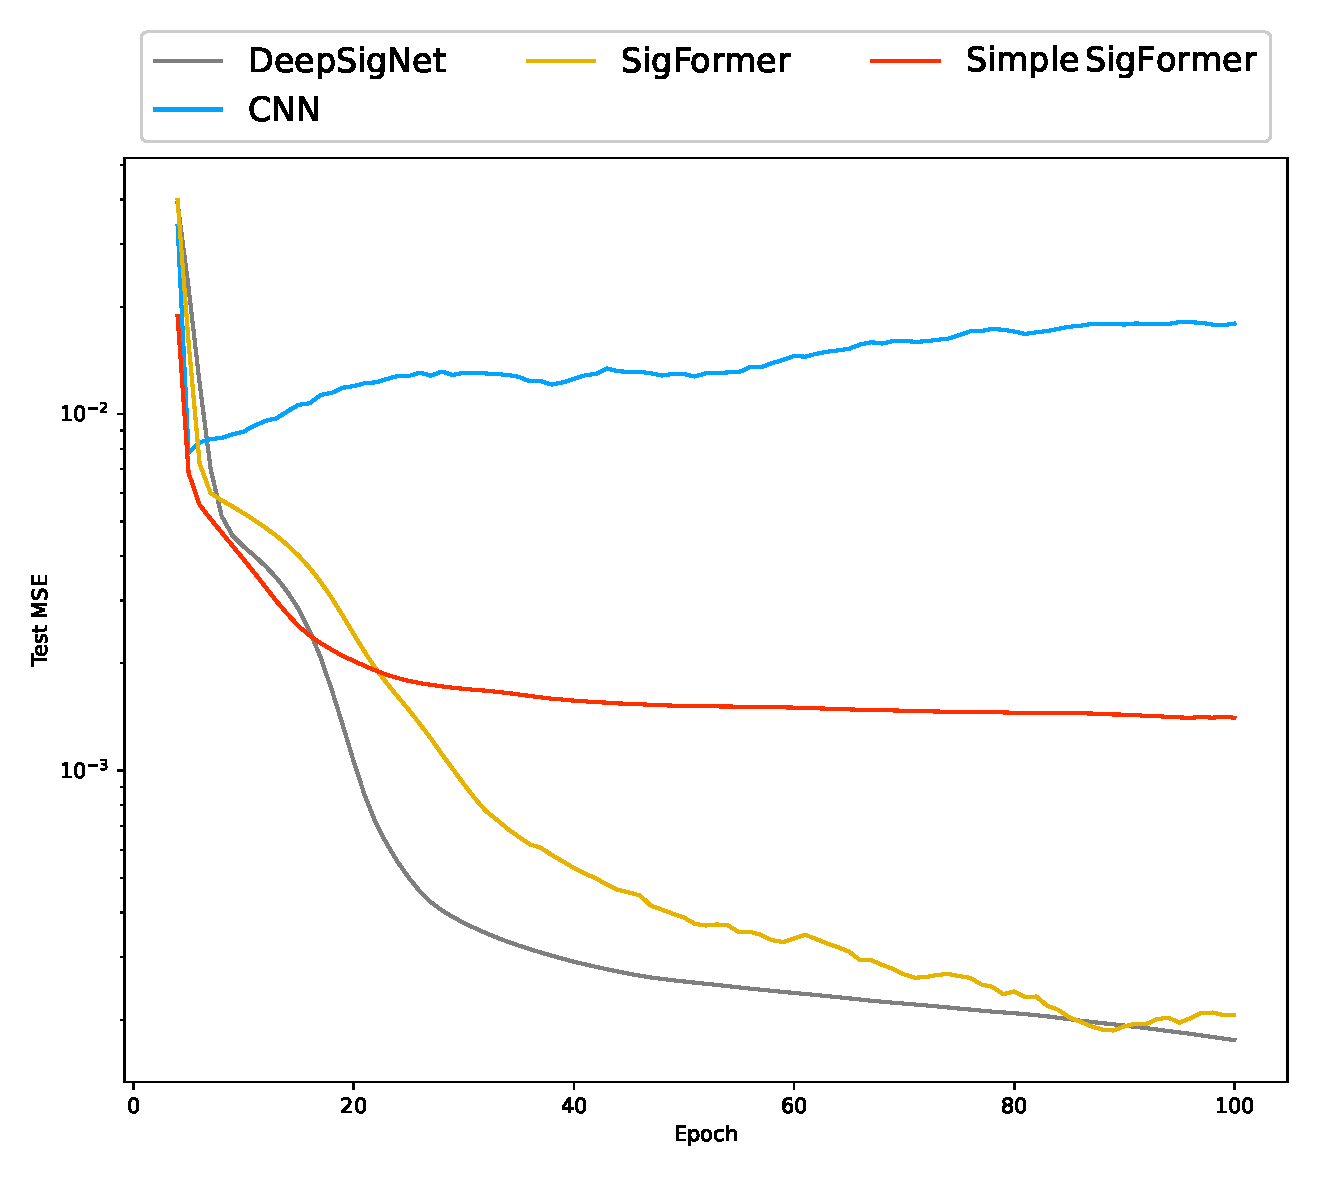
\includegraphics[width=0.32\textwidth]{fig//fBm_grid=100_Hbeta.eps}
			
\includegraphics[width=0.32\textwidth]{fig//rBergomi_grid=100_Hbeta_eta=1_v0=0.01.eps}
			
\includegraphics[width=0.32\textwidth]{fig//rHeston_grid=100_Hbeta_kappa1=0.1_kappa2=0.03_theta=0.3_v0=0.01.eps}}
		}
		\caption{Loss plot for (Left:) fBms; (Middle:) rBergomi volatility processes; (Right:) rHeston volatility processes with input lengths equal to $100$. The data has been taken the rolling mean with a window size of 5.}
	\end{figure}
	
	\begin{figure}[H]
		\centering
		\resizebox{0.9\textwidth}{!}{
		\subfigure[$H\sim\text{Uniform}(0,0.5)$]{
			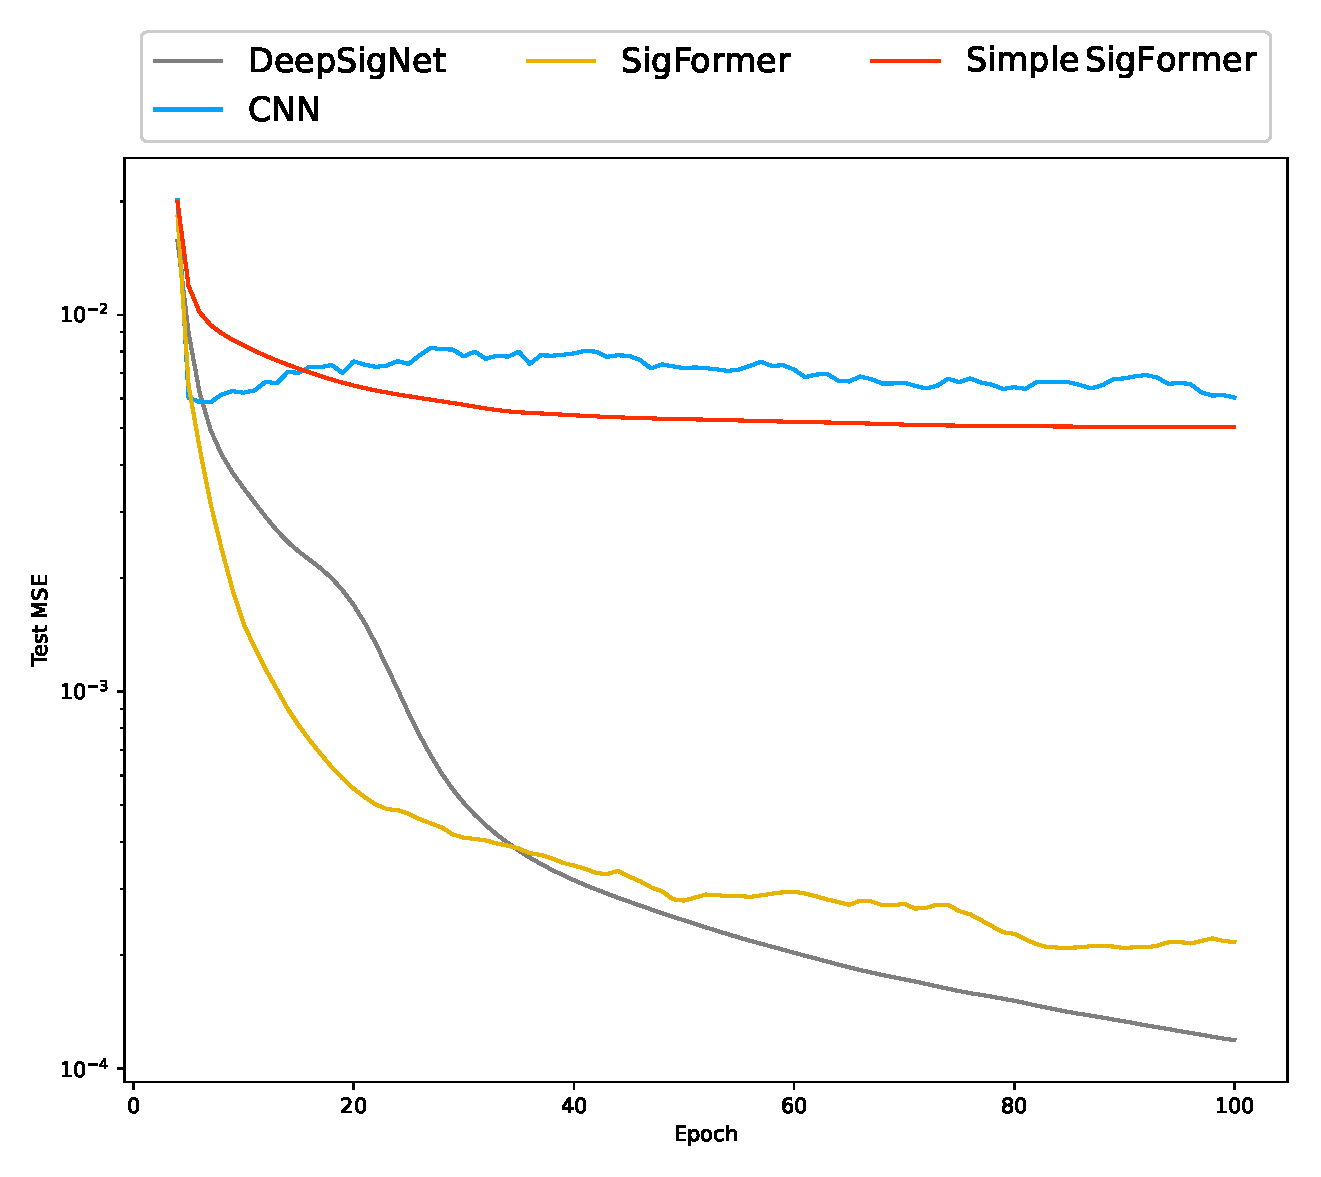
\includegraphics[width=0.32\textwidth]{fig//fBm_grid=200_Huniform.eps}
			
\includegraphics[width=0.32\textwidth]{fig//rBergomi_grid=200_Huniform_eta=1_v0=0.01.eps}
			
\includegraphics[width=0.32\textwidth]{fig//rHeston_grid=200_Huniform_kappa1=0.1_kappa2=0.03_theta=0.3_v0=0.01.eps}}
		}
		\resizebox{0.9\textwidth}{!}{
		\subfigure[$H\sim\text{Beta}(1,\,9)$]{
			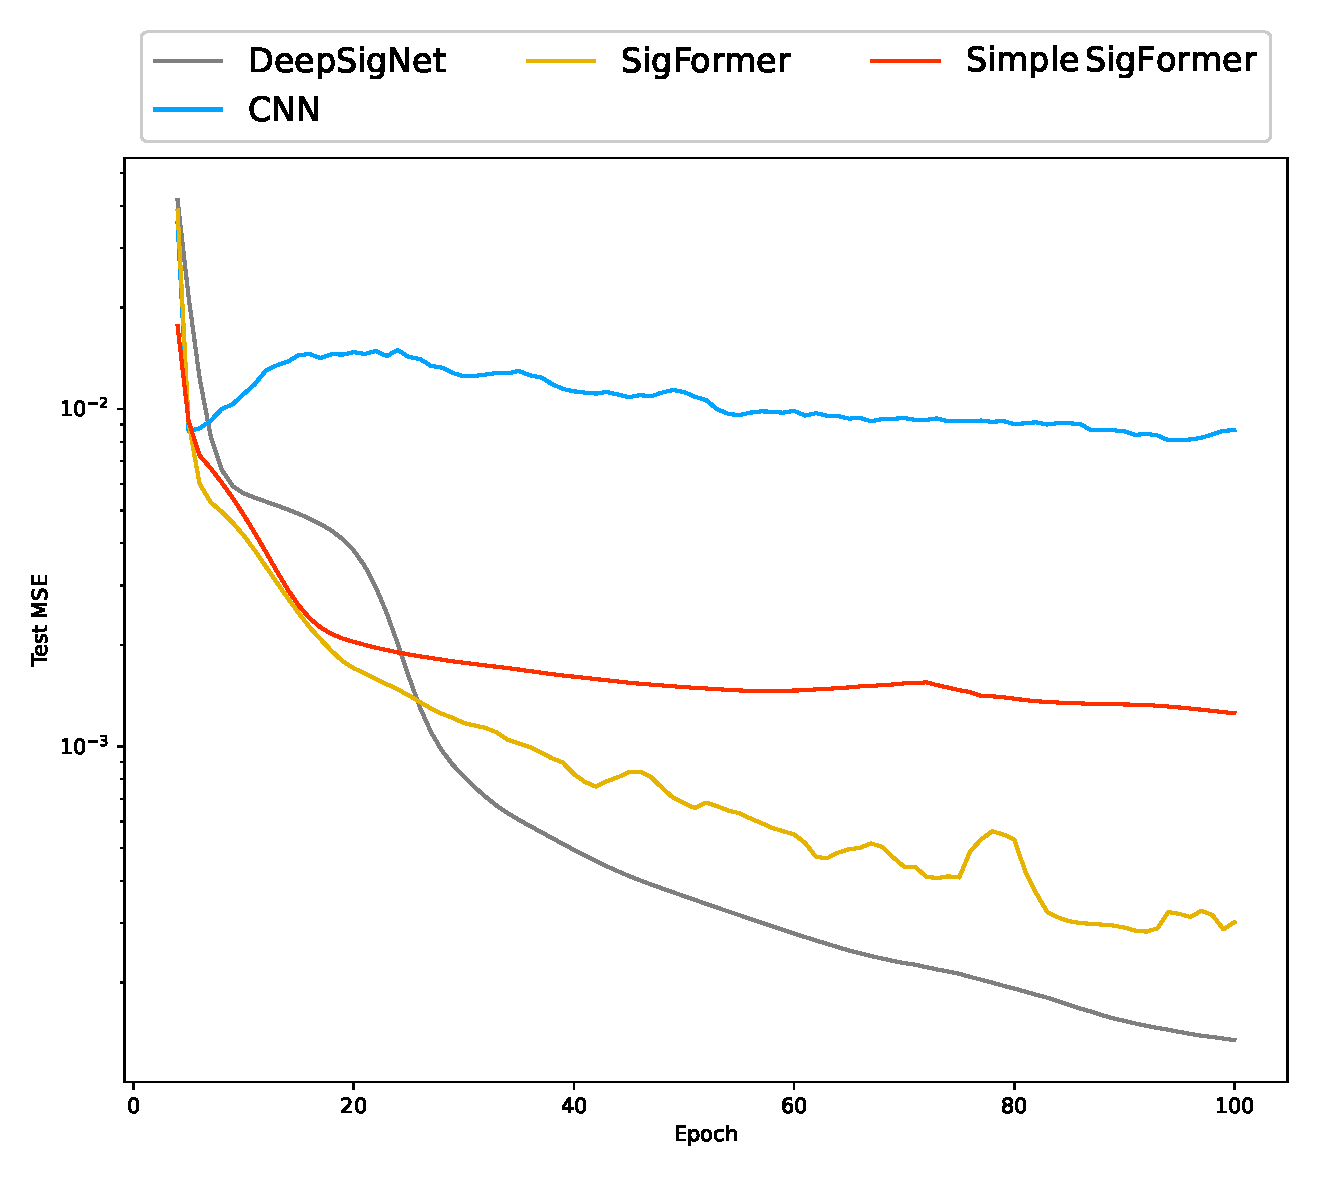
\includegraphics[width=0.32\textwidth]{fig//fBm_grid=200_Hbeta.eps}
			
\includegraphics[width=0.32\textwidth]{fig//rBergomi_grid=200_Hbeta_eta=1_v0=0.01.eps}
			
\includegraphics[width=0.32\textwidth]{fig//rHeston_grid=200_Hbeta_kappa1=0.1_kappa2=0.03_theta=0.3_v0=0.01.eps}}
		}
		\caption{Loss plot for (Left:) fBms; (Middle:) rBergomi volatility processes; (Right:) rHeston volatility processes with input lengths equal to $200$. The data has been taken the rolling mean with a window size of 5.}
	\end{figure}
	
	\begin{figure}[H]
		\centering
		\resizebox{0.9\textwidth}{!}{
		\subfigure[$H\sim\text{Uniform}(0,0.5)$]{
			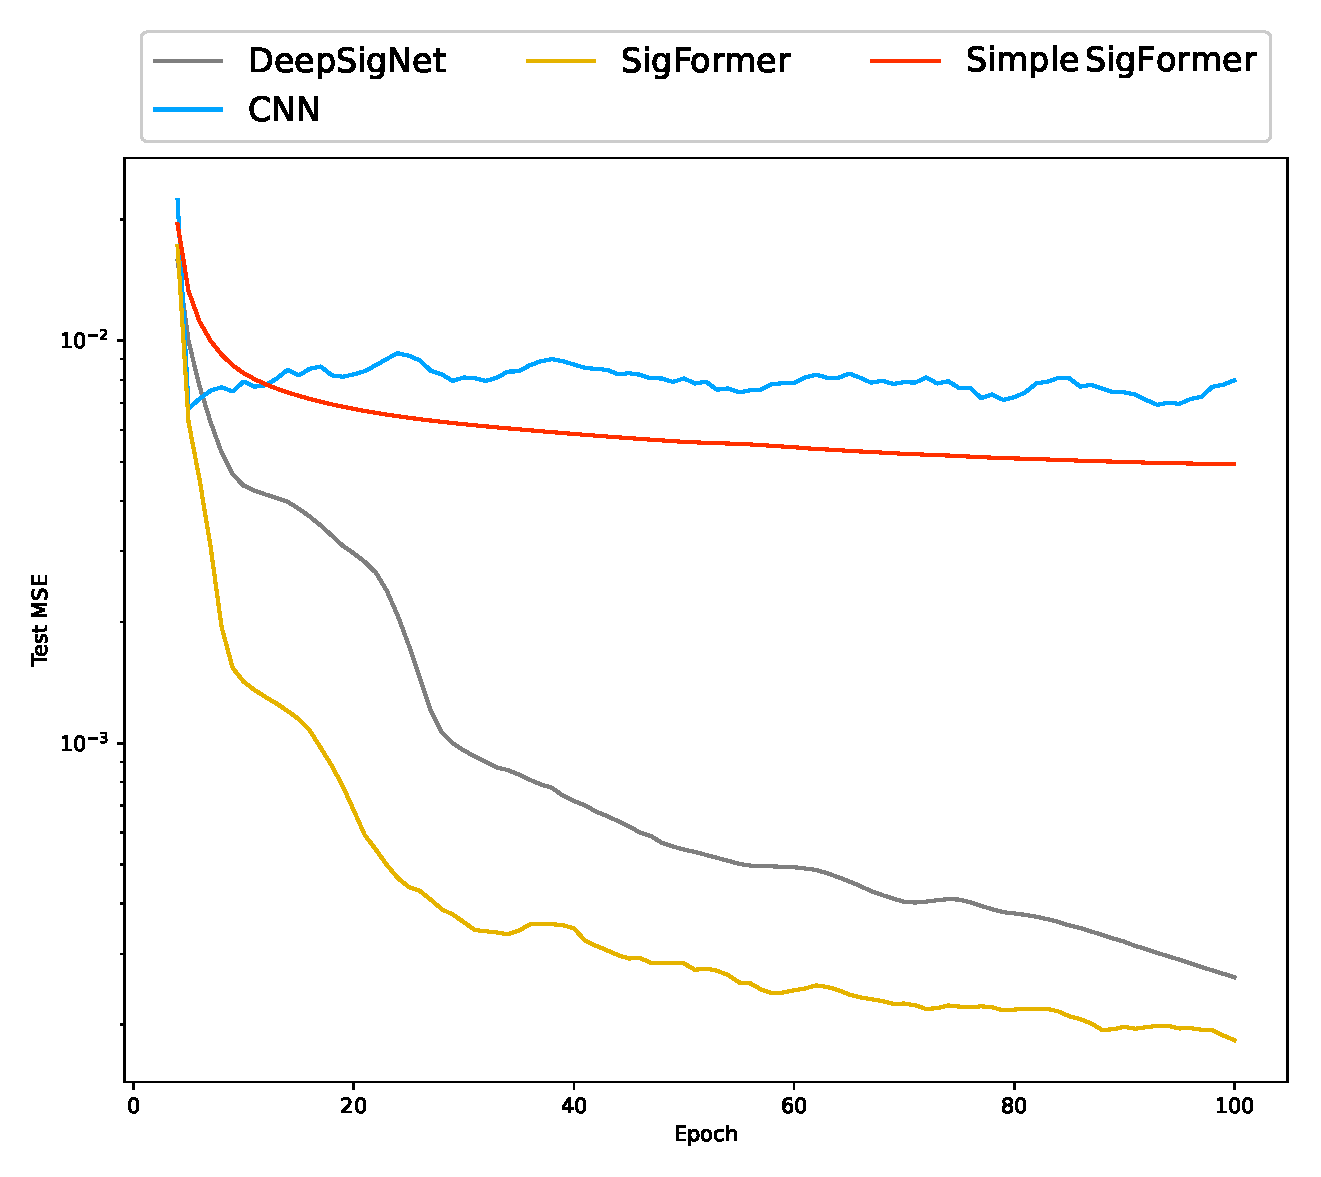
\includegraphics[width=0.32\textwidth]{fig//fBm_grid=300_Huniform.eps}
			
\includegraphics[width=0.32\textwidth]{fig//rBergomi_grid=300_Huniform_eta=1_v0=0.01.eps}
			
\includegraphics[width=0.32\textwidth]{fig//rHeston_grid=300_Huniform_kappa1=0.1_kappa2=0.03_theta=0.3_v0=0.01.eps}}
		}
		\resizebox{0.9\textwidth}{!}{
		\subfigure[$H\sim\text{Beta}(1,\,9)$]{
			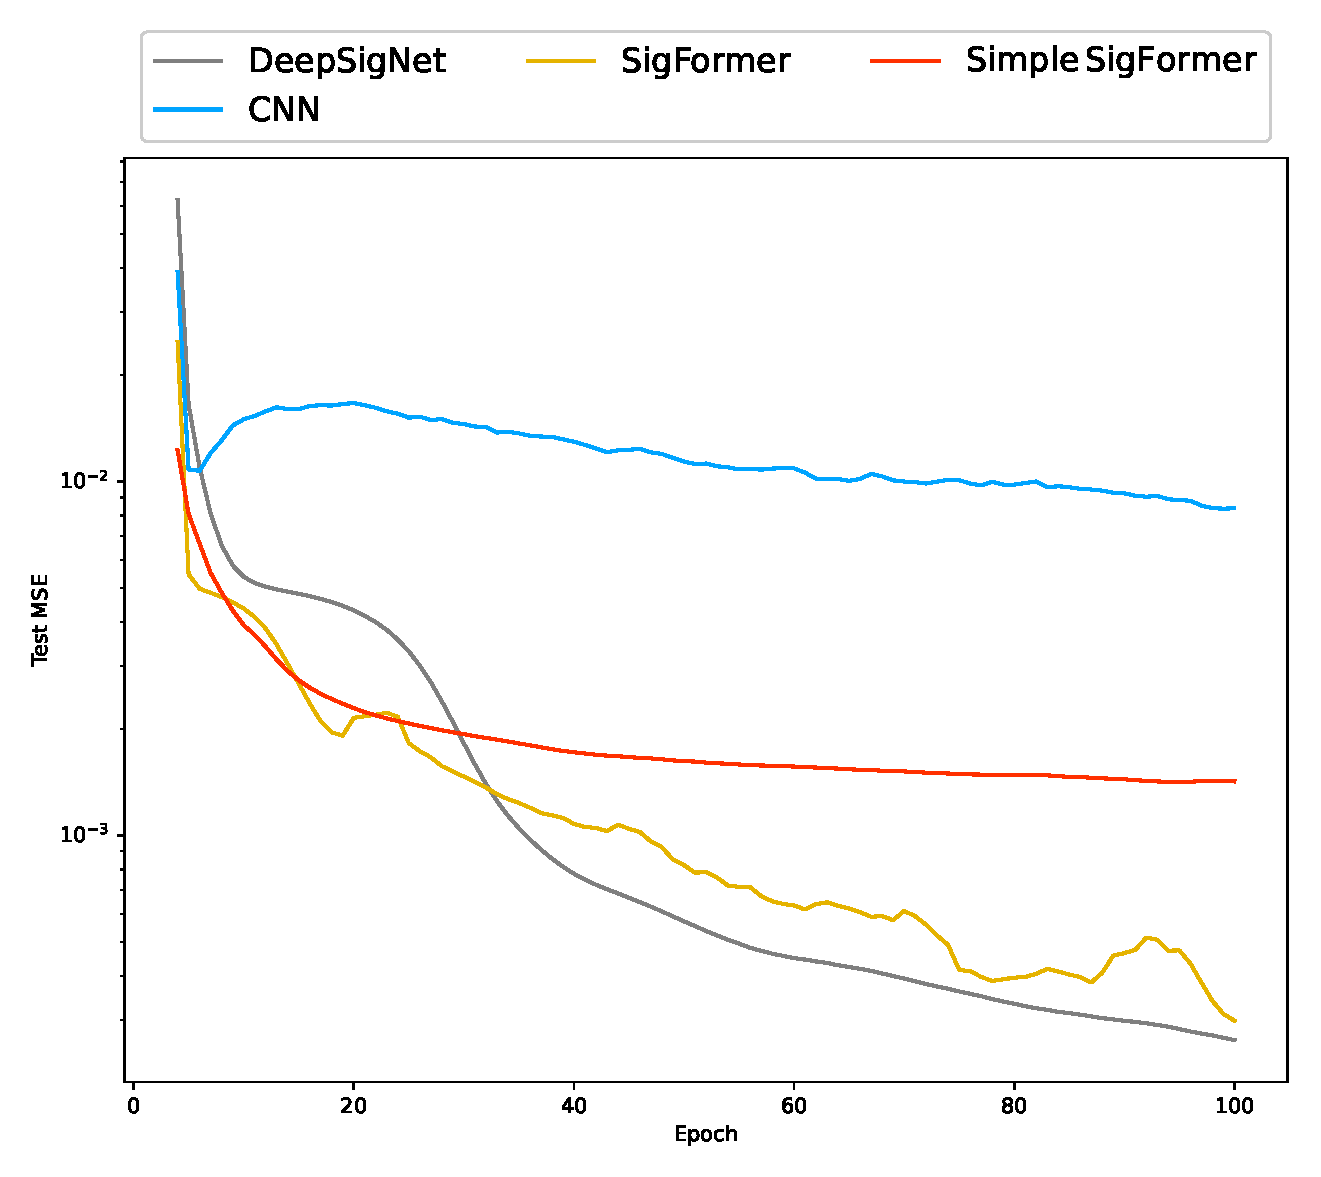
\includegraphics[width=0.32\textwidth]{fig//fBm_grid=300_Hbeta.eps}
			
\includegraphics[width=0.32\textwidth]{fig//rBergomi_grid=300_Hbeta_eta=1_v0=0.01.eps}
			
\includegraphics[width=0.32\textwidth]{fig//rHeston_grid=300_Hbeta_kappa1=0.1_kappa2=0.03_theta=0.3_v0=0.01.eps}}
		}
		\caption{Loss plot for (Left:) fBms; (Middle:) rBergomi volatility processes; (Right:) rHeston volatility processes with input lengths equal to $300$. The data has been taken the rolling mean with a window size of 5.}
	\end{figure}
	
	\begin{figure}[H]
		\centering
		\resizebox{0.9\textwidth}{!}{
		\subfigure[$H\sim\text{Uniform}(0,0.5)$]{
			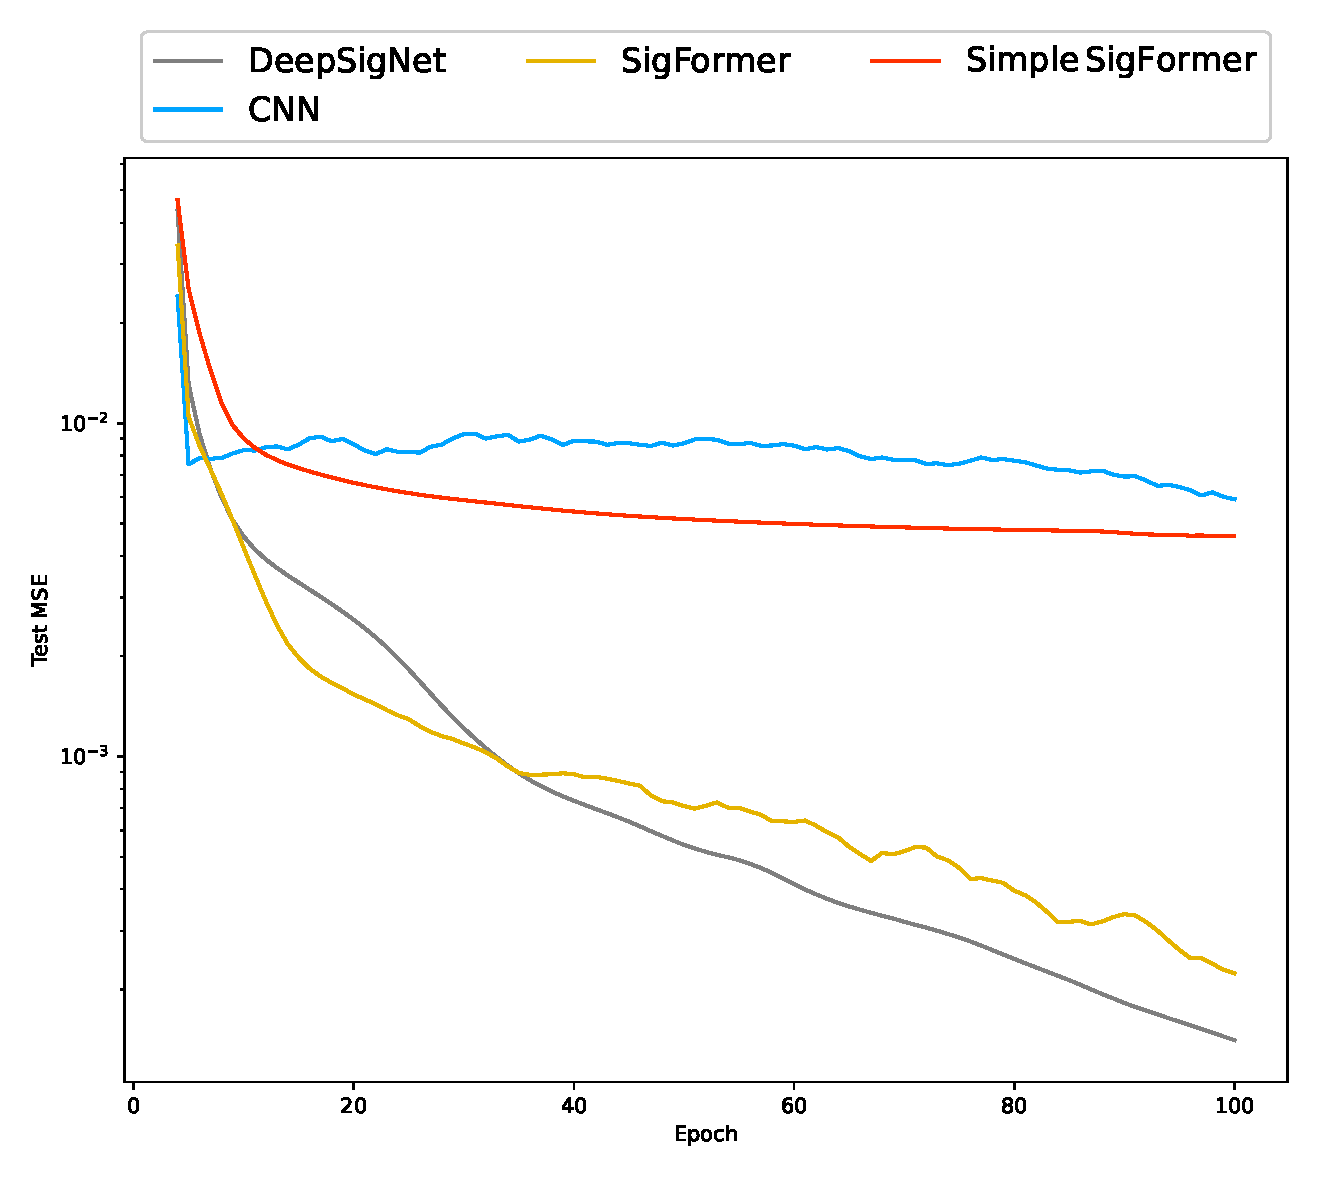
\includegraphics[width=0.32\textwidth]{fig//fBm_grid=400_Huniform.eps}
			
\includegraphics[width=0.32\textwidth]{fig//rBergomi_grid=400_Huniform_eta=1_v0=0.01.eps}
			
\includegraphics[width=0.32\textwidth]{fig//rHeston_grid=400_Huniform_kappa1=0.1_kappa2=0.03_theta=0.3_v0=0.01.eps}}
		}
		\resizebox{0.9\textwidth}{!}{
		\subfigure[$H\sim\text{Beta}(1,\,9)$]{
			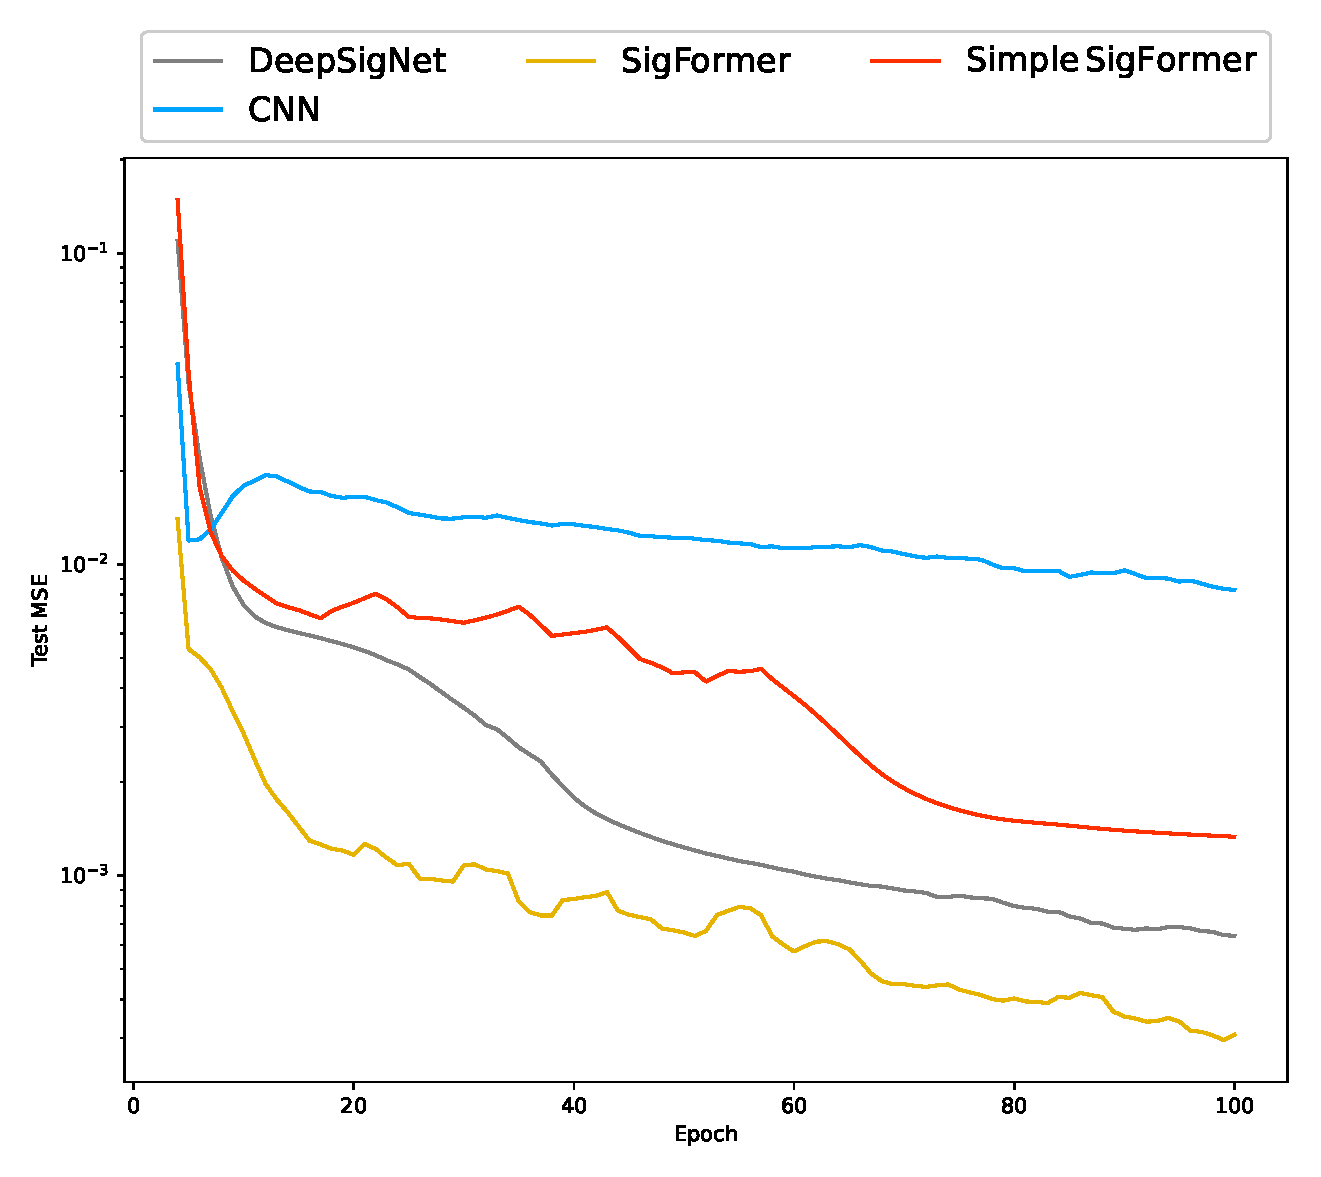
\includegraphics[width=0.32\textwidth]{fig//fBm_grid=400_Hbeta.eps}
			
\includegraphics[width=0.32\textwidth]{fig//rBergomi_grid=400_Hbeta_eta=1_v0=0.01.eps}
			
\includegraphics[width=0.32\textwidth]{fig//rHeston_grid=400_Hbeta_kappa1=0.1_kappa2=0.03_theta=0.3_v0=0.01.eps}}
		}
		\caption{Loss plot for (Left:) fBms; (Middle:) rBergomi volatility processes; (Right:) rHeston volatility processes with input lengths equal to $400$. The data has been taken the rolling mean with a window size of 5.}
	\end{figure}
	
	\begin{figure}[H]
		\centering
		\resizebox{0.9\textwidth}{!}{
		\subfigure[$H\sim\text{Uniform}(0,0.5)$]{
			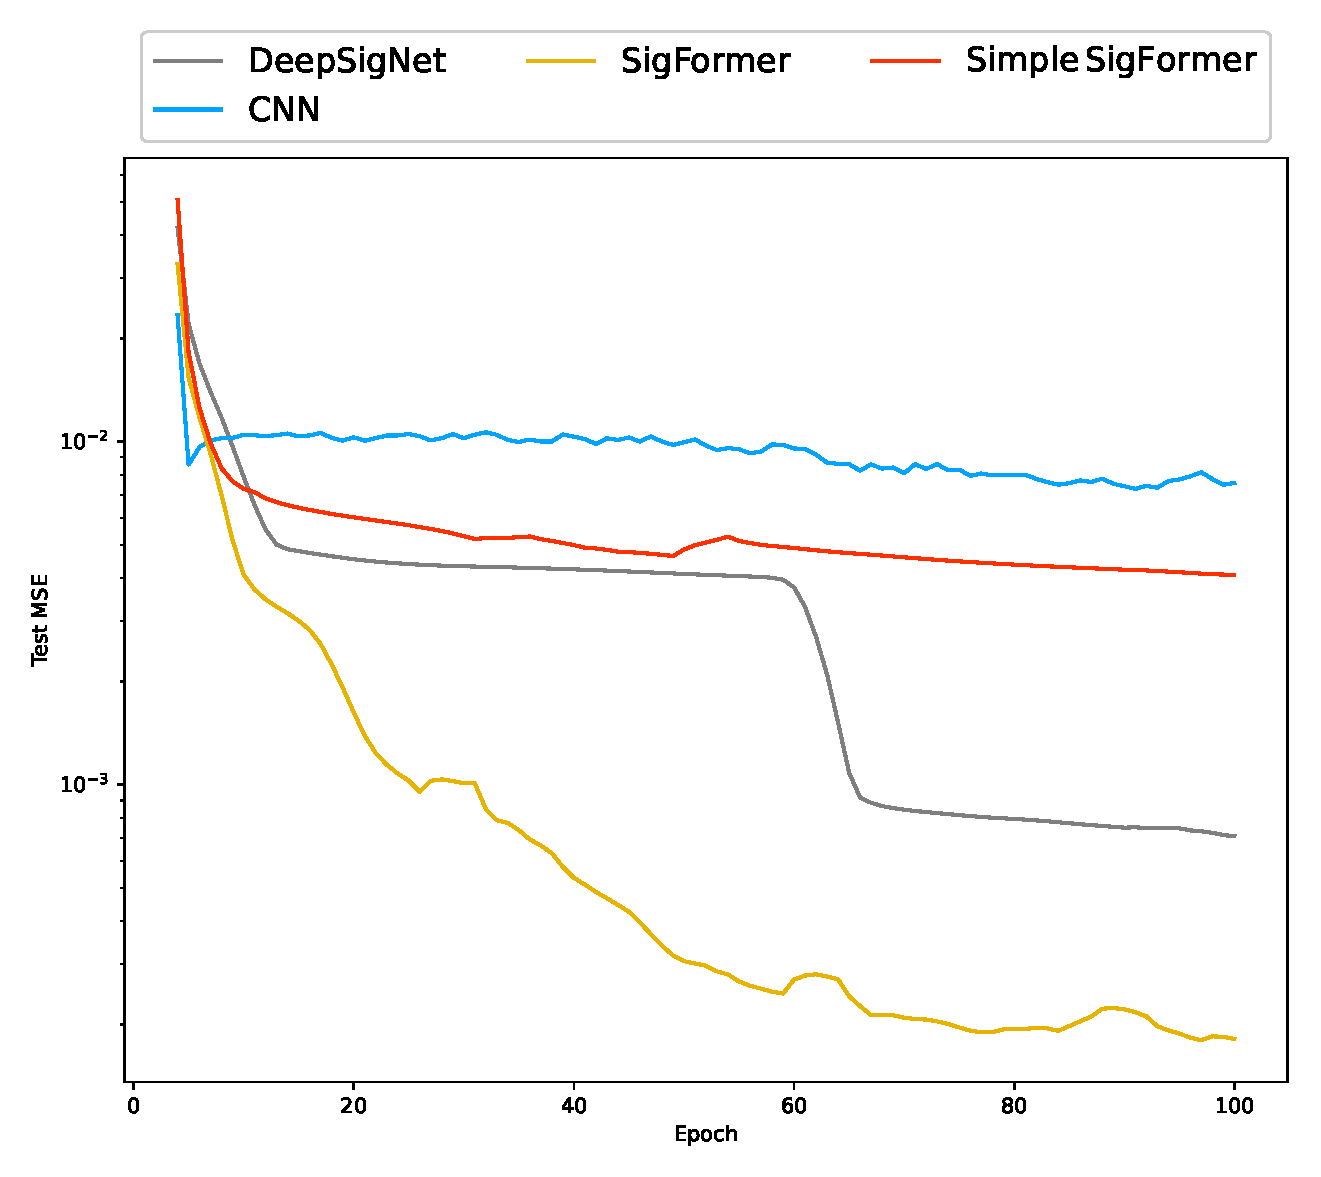
\includegraphics[width=0.32\textwidth]{fig//fBm_grid=500_Huniform.eps}
			
\includegraphics[width=0.32\textwidth]{fig//rBergomi_grid=500_Huniform_eta=1_v0=0.01.eps}
			
\includegraphics[width=0.32\textwidth]{fig//rHeston_grid=500_Huniform_kappa1=0.1_kappa2=0.03_theta=0.3_v0=0.01.eps}}
		}
		\resizebox{0.9\textwidth}{!}{
		\subfigure[$H\sim\text{Beta}(1,\,9)$]{
			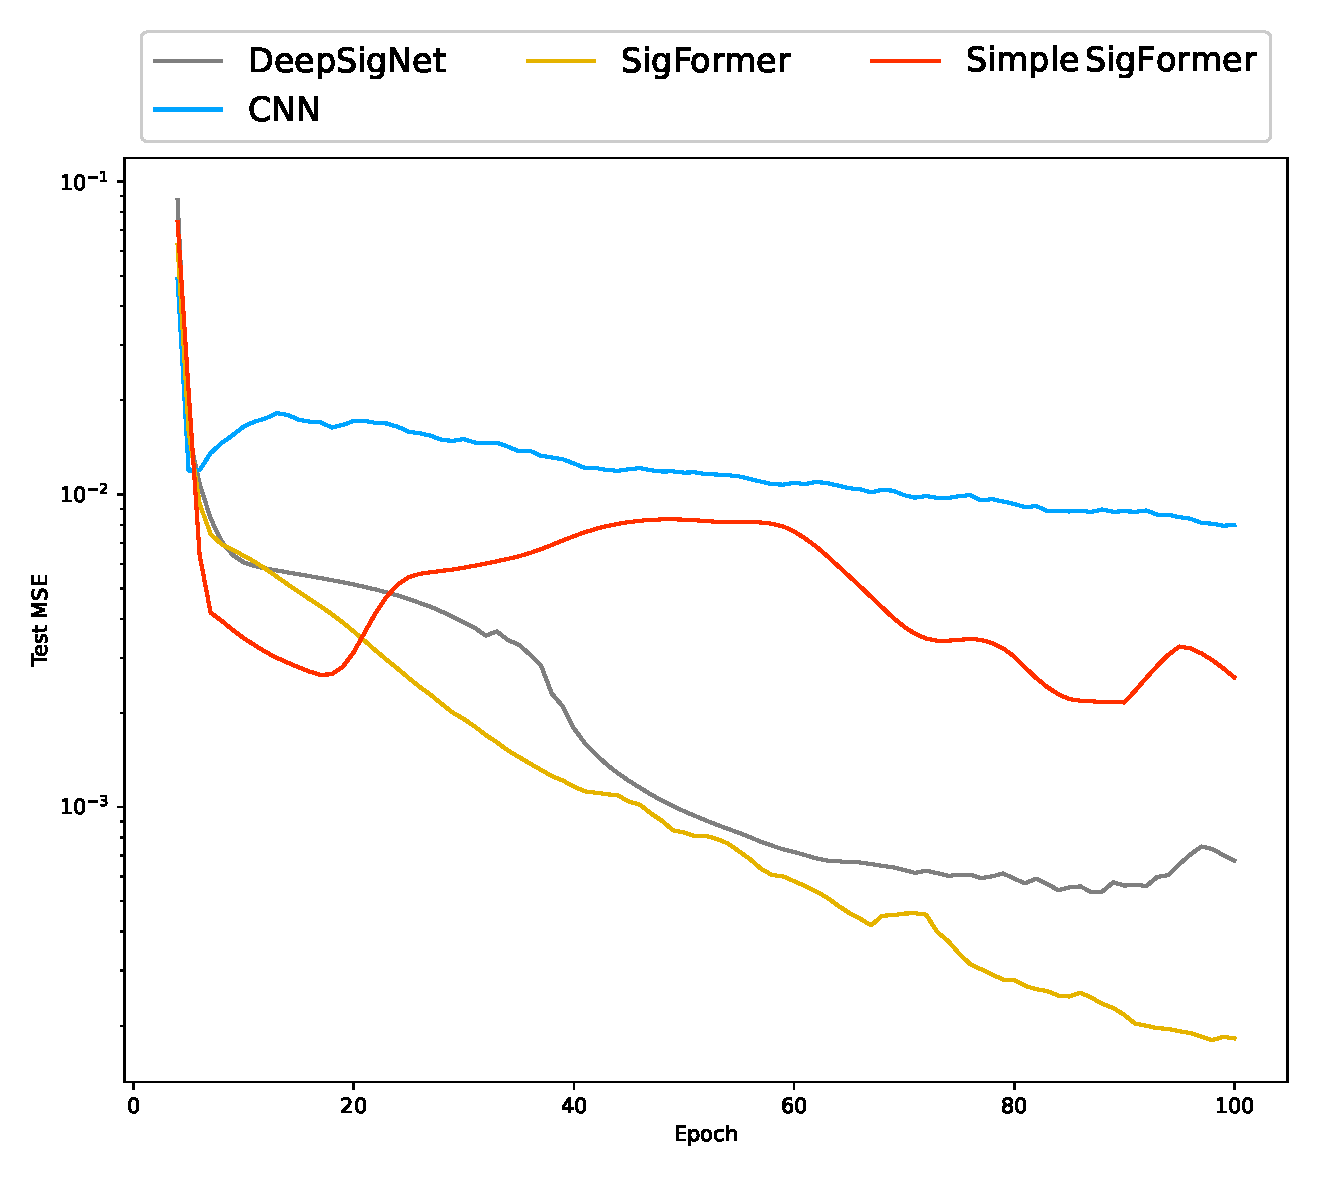
\includegraphics[width=0.32\textwidth]{fig//fBm_grid=500_Hbeta.eps}
			
\includegraphics[width=0.32\textwidth]{fig//rBergomi_grid=500_Hbeta_eta=1_v0=0.01.eps}
			
\includegraphics[width=0.32\textwidth]{fig//rHeston_grid=500_Hbeta_kappa1=0.1_kappa2=0.03_theta=0.3_v0=0.01.eps}}
		}
		\caption{Loss plot for (Left:) fBms; (Middle:) rBergomi volatility processes; (Right:) rHeston volatility processes with input lengths equal to $500$. The data has been taken the rolling mean with a window size of 5.}
	\end{figure}

	\subsection{Loss plots for different models with the signature truncation order varying from $1$ to $5$}
	\label{subapdix-loss-plots-truncation}
	\begin{figure}[H]
		\centering
		\subfigure{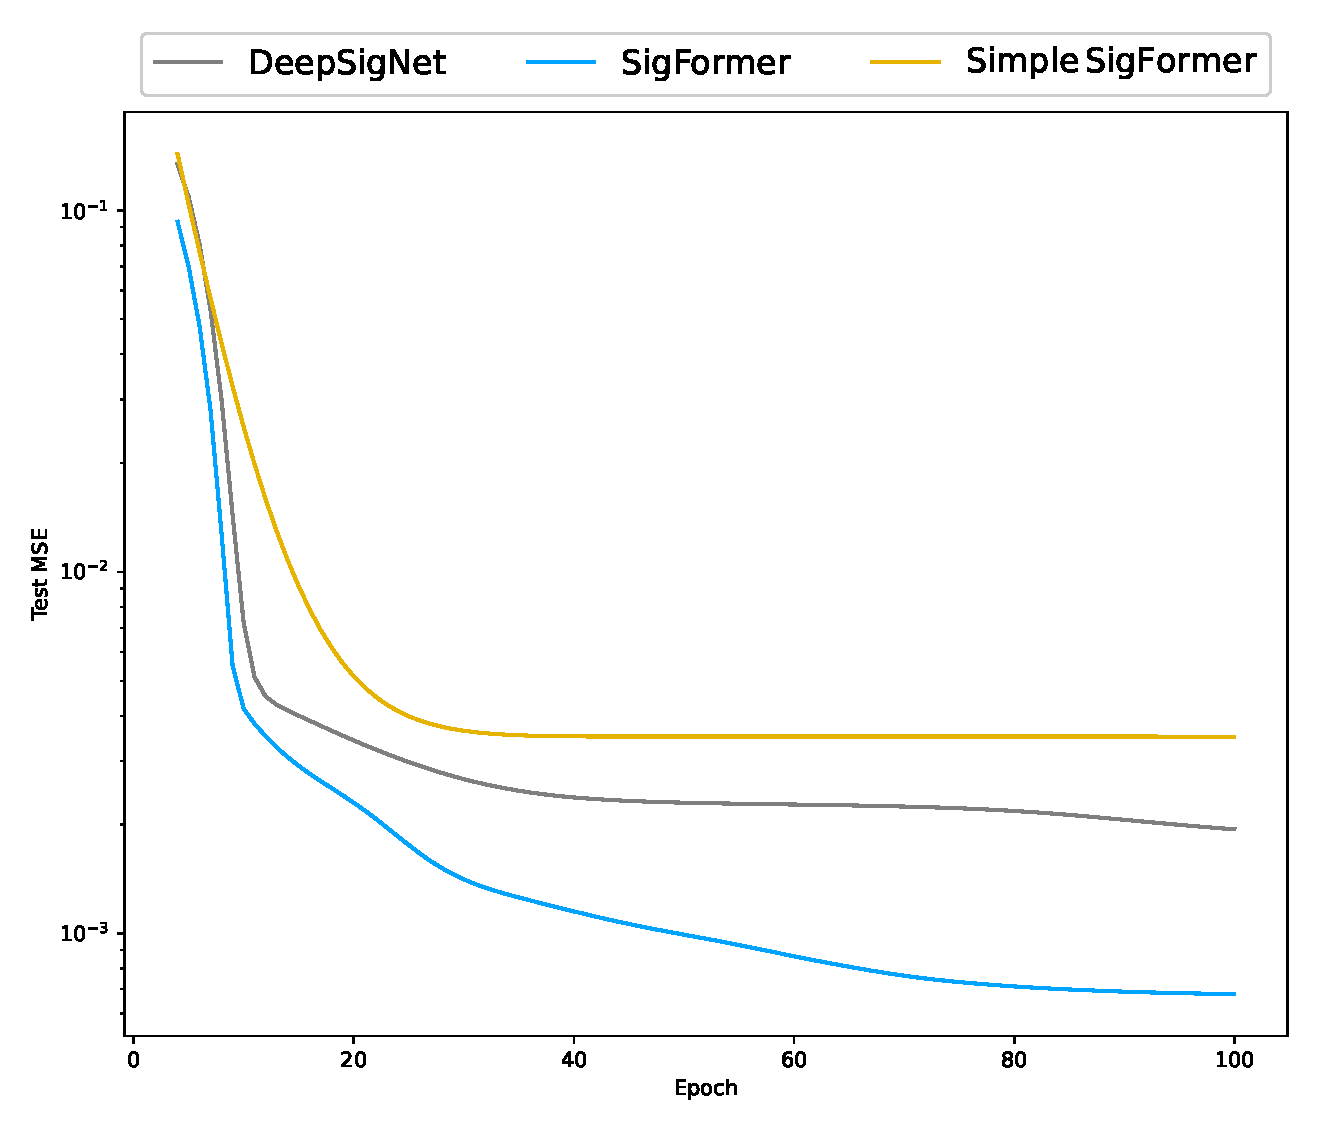
\includegraphics[width=0.30\textwidth]{fig//fBm_grid=100_Hbeta_Trun1.eps}}
		\subfigure{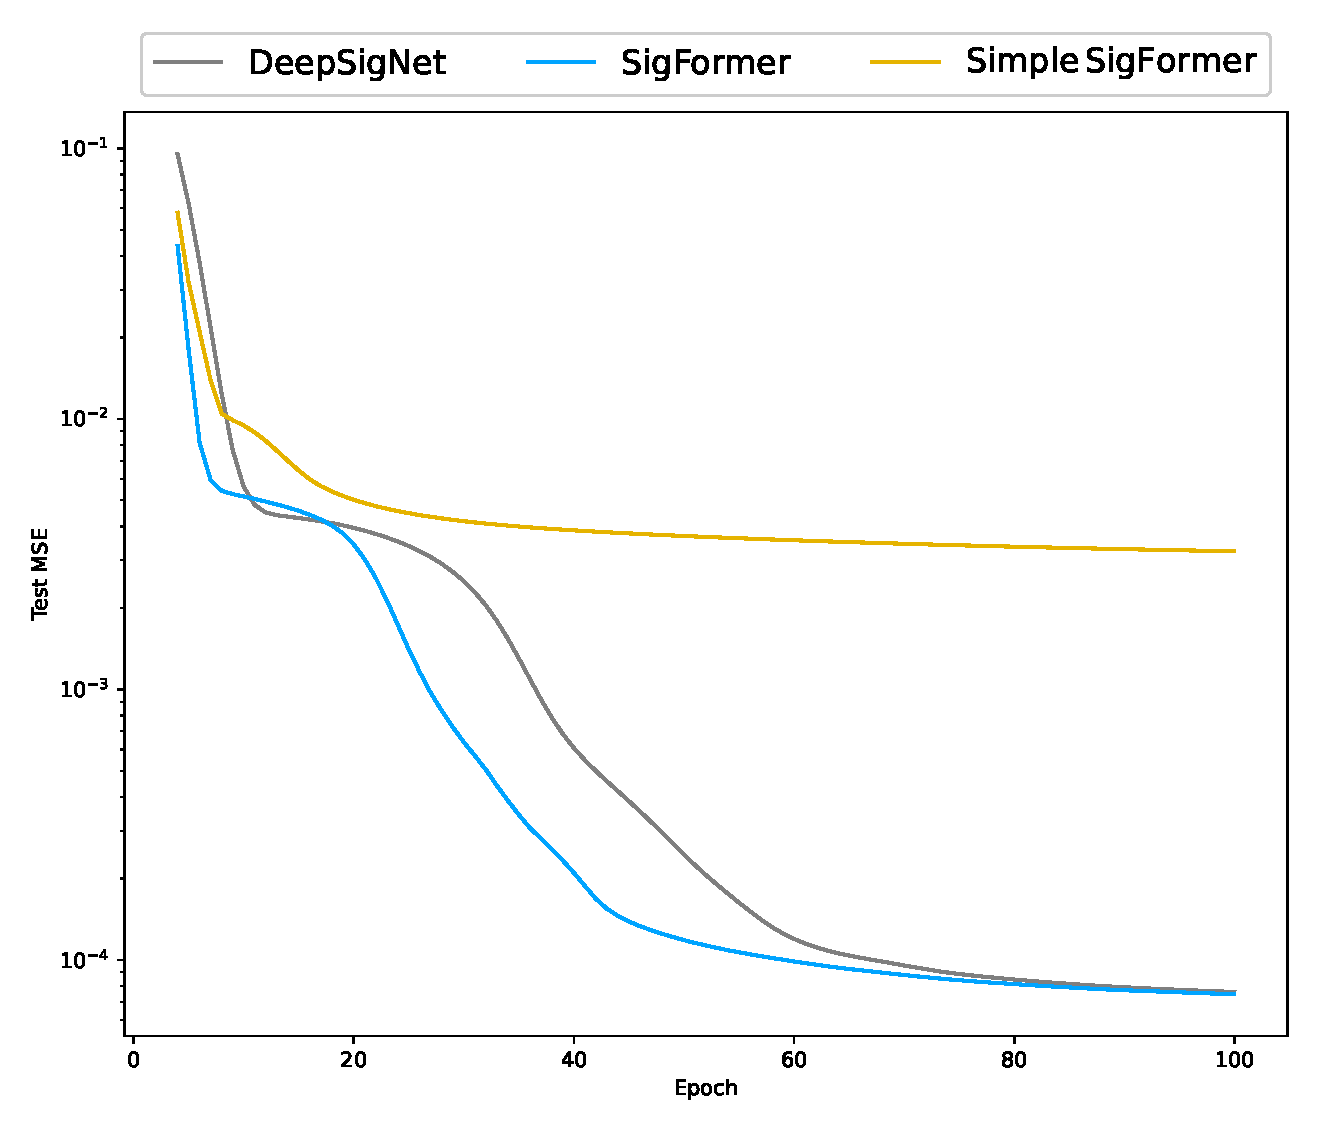
\includegraphics[width=0.30\textwidth]{fig//fBm_grid=100_Hbeta_Trun2.eps}}
		\subfigure{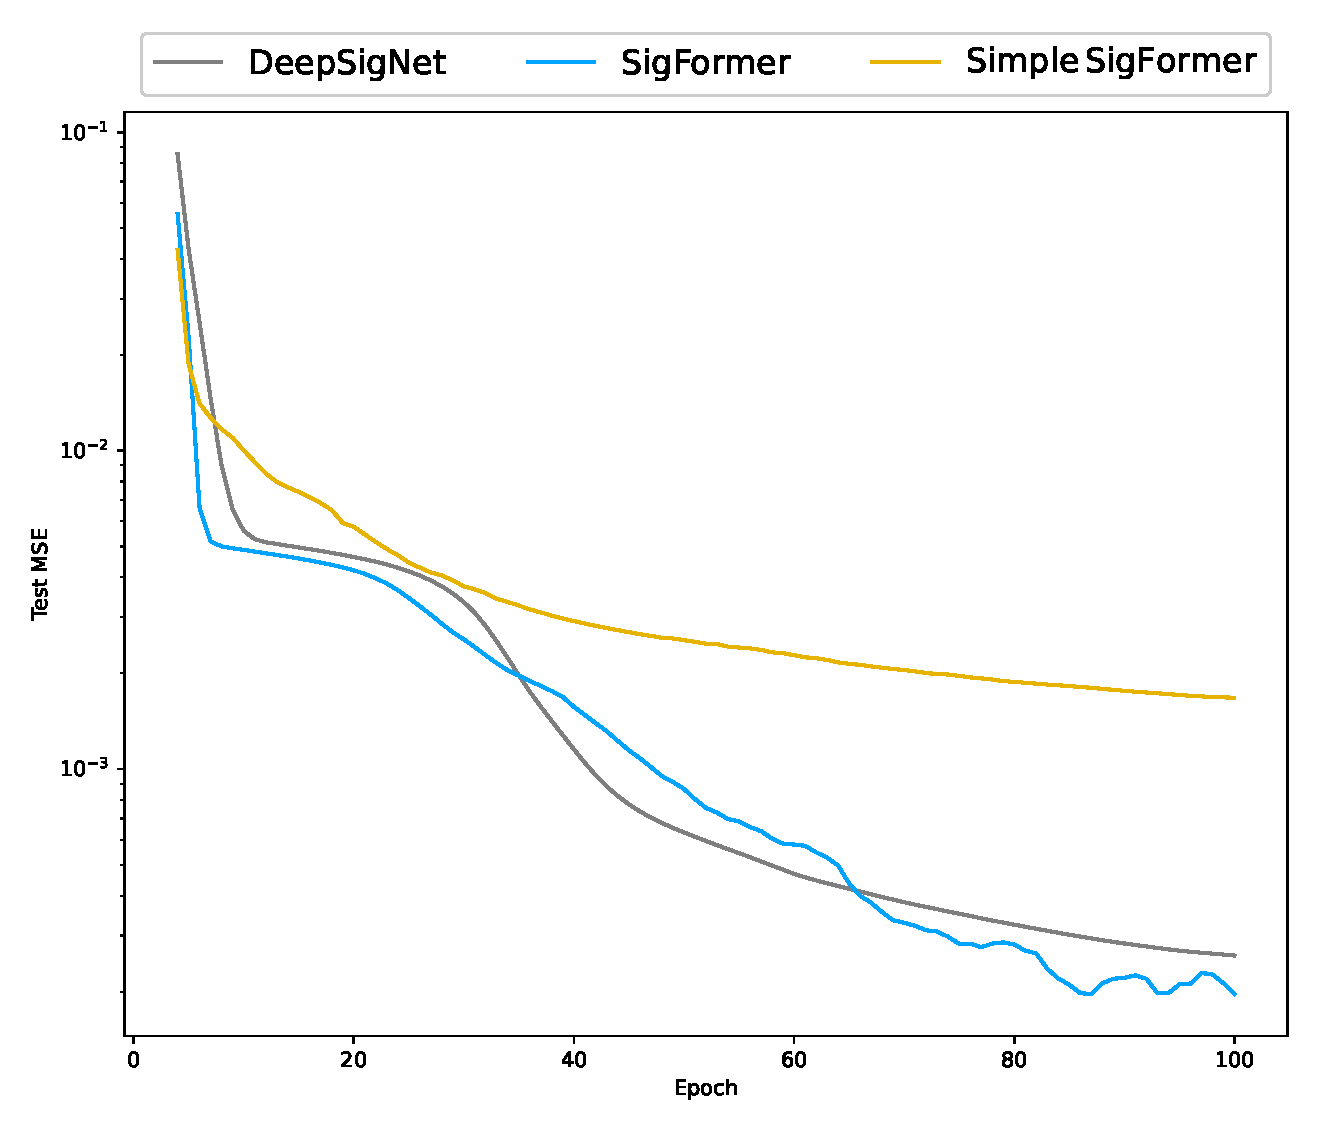
\includegraphics[width=0.30\textwidth]{fig//fBm_grid=100_Hbeta_Trun3.eps}}
		\subfigure{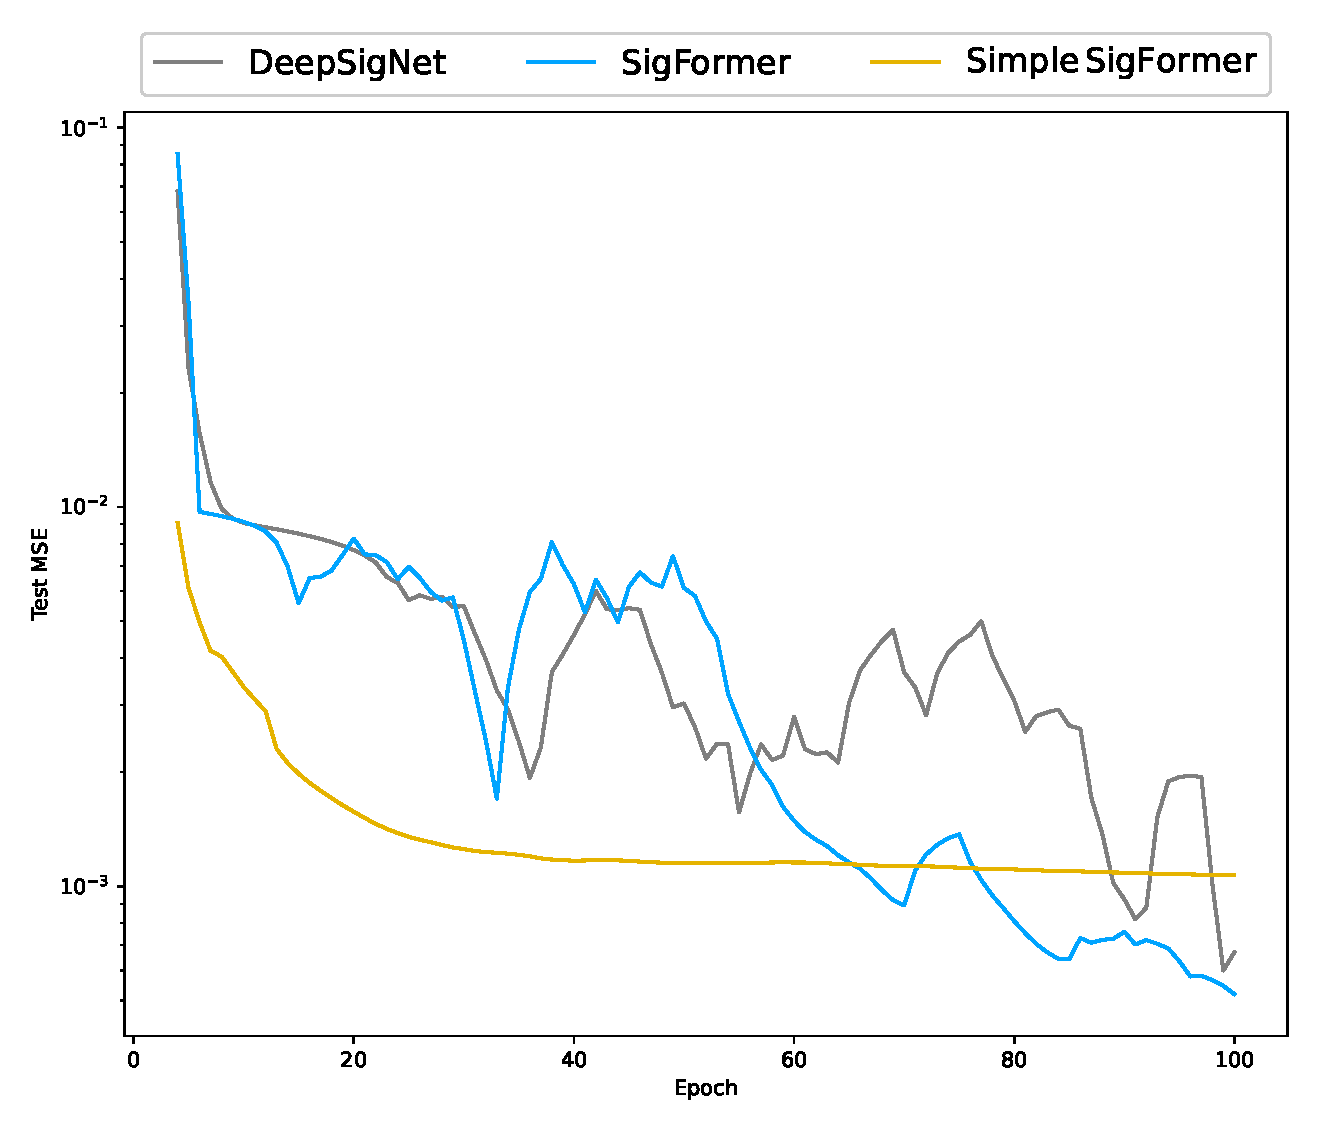
\includegraphics[width=0.30\textwidth]{fig//fBm_grid=100_Hbeta_Trun4.eps}}
		\subfigure{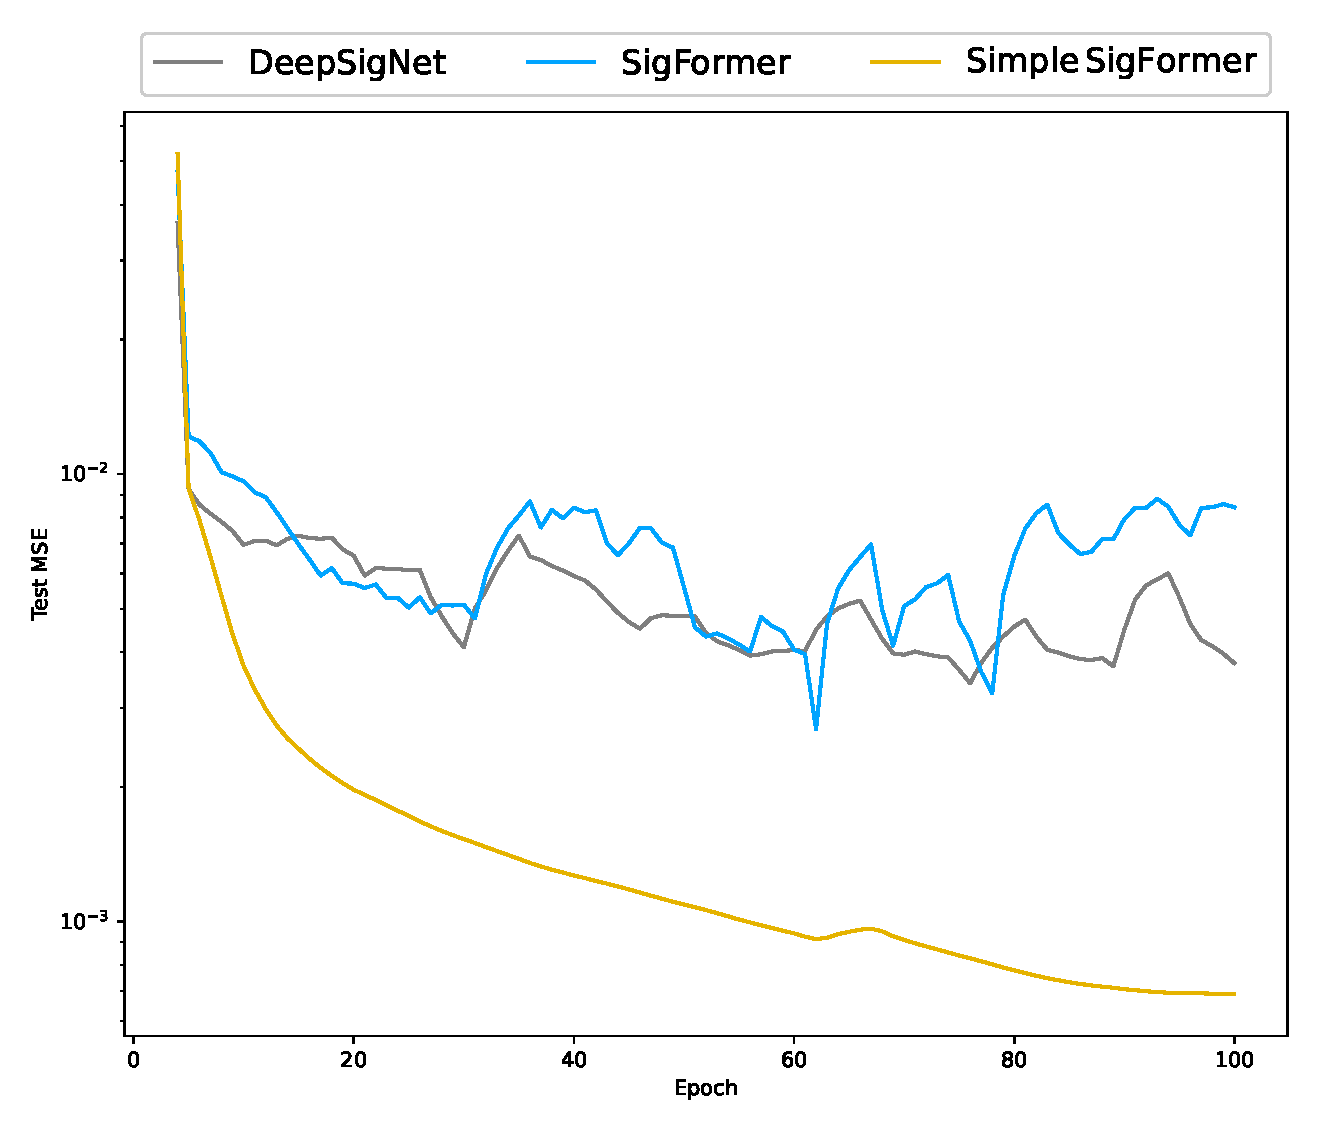
\includegraphics[width=0.30\textwidth]{fig//fBm_grid=100_Hbeta_Trun5.eps}}
		\caption{Loss plot for fBms with signature truncation order ranging from (left to right and top to bottom:) $\{1,\,2,\,3,\,4,\,5\}$. Here $H\sim\text{Beta}(1,\,9)$ and the input lengths equal to $100$. The data has been taken the rolling mean with a window size of 5.}
	\end{figure}
	
	\begin{figure}[H]
		\centering
 		\subfigure{
\includegraphics[width=0.30\textwidth]{fig//rBergomi_grid=100_Hbeta_eta=1_v0=0.01_Trun1.eps}}
		\subfigure{
\includegraphics[width=0.30\textwidth]{fig//rBergomi_grid=100_Hbeta_eta=1_v0=0.01_Trun2.eps}}
		\subfigure{
\includegraphics[width=0.30\textwidth]{fig//rBergomi_grid=100_Hbeta_eta=1_v0=0.01_Trun3.eps}}
		\subfigure{
\includegraphics[width=0.30\textwidth]{fig//rBergomi_grid=100_Hbeta_eta=1_v0=0.01_Trun4.eps}}
		\subfigure{
\includegraphics[width=0.30\textwidth]{fig//rBergomi_grid=100_Hbeta_eta=1_v0=0.01_Trun5.eps}}
		\caption{Loss plot for rBergomi volatility processes with signature truncation order ranging from (left to right and top to bottom:) $\{1,\,2,\,3,\,4,\,5\}$. Here $H\sim\text{Beta}(1,\,9)$ and the input lengths equal to $100$. The data has been taken the rolling mean with a window size of 5.}
	\end{figure}
	
	\begin{figure}[H]
		\centering
		\subfigure{
\includegraphics[width=0.30\textwidth]{fig//rHeston_grid=100_Hbeta_kappa1=0.1_kappa2=0.03_theta=0.3_v0=0.01_Trun1.eps}}
		\subfigure{
\includegraphics[width=0.30\textwidth]{fig//rHeston_grid=100_Hbeta_kappa1=0.1_kappa2=0.03_theta=0.3_v0=0.01_Trun2.eps}}
		\subfigure{
\includegraphics[width=0.30\textwidth]{fig//rHeston_grid=100_Hbeta_kappa1=0.1_kappa2=0.03_theta=0.3_v0=0.01_Trun3.eps}}
		\subfigure{
\includegraphics[width=0.30\textwidth]{fig//rHeston_grid=100_Hbeta_kappa1=0.1_kappa2=0.03_theta=0.3_v0=0.01_Trun4.eps}}
		\subfigure{
\includegraphics[width=0.30\textwidth]{fig//rHeston_grid=100_Hbeta_kappa1=0.1_kappa2=0.03_theta=0.3_v0=0.01_Trun5.eps}}
		\caption{Loss plot for rHeston volatility processes with signature truncation order ranging from (left to right and top to bottom:) $\{1,\,2,\,3,\,4,\,5,\,6\}$. Here $H\sim\text{Beta}(1,\,9)$ and the input lengths equal to $100$. The data has been taken the rolling mean with a window size of 5.}
	\end{figure}
	
	
	
	\subsection{Loss plots for multiple parameters calibrations}
	\label{subapdix-loss-plots-multiple}
	\begin{figure}[H]
		\centering
		
\includegraphics[width=0.45\textwidth]{fig//rBergomi_grid=100_Hbeta_etauniform_v0=0.01.eps}
		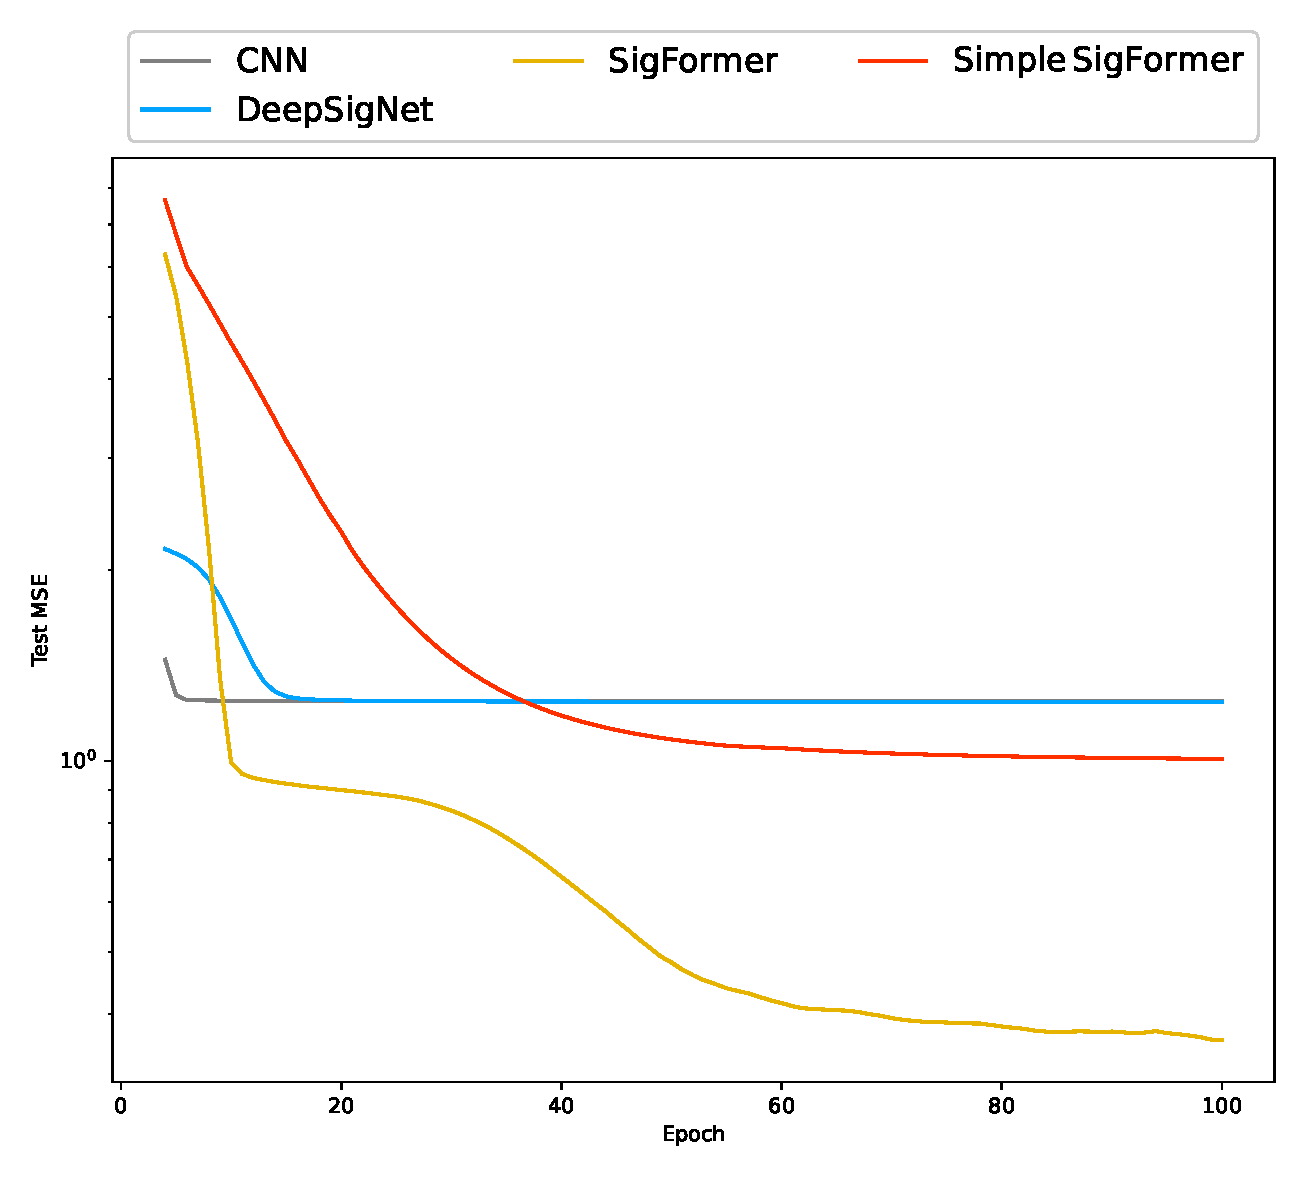
\includegraphics[width=0.45\textwidth]{fig//rHeston_grid=100_Hbeta_kappa1=0.1_kappa2uniform_theta=0.3_v0=0.01.eps}
		\caption{Loss plot of two parameters calibration for (Left:) rBergomi volatility processes and (Right:) rHeston volatility processes with $H\sim\text{Beta}(1,\,9)$, $\eta\sim\text{Uniform}(0,\,3)$ and $\kappa_2\sim\text{Uniform}(0,\,3)$. The data has been taken the rolling mean with a window size of 5.}
	\end{figure}
	
	\begin{figure}[H]
		\centering
		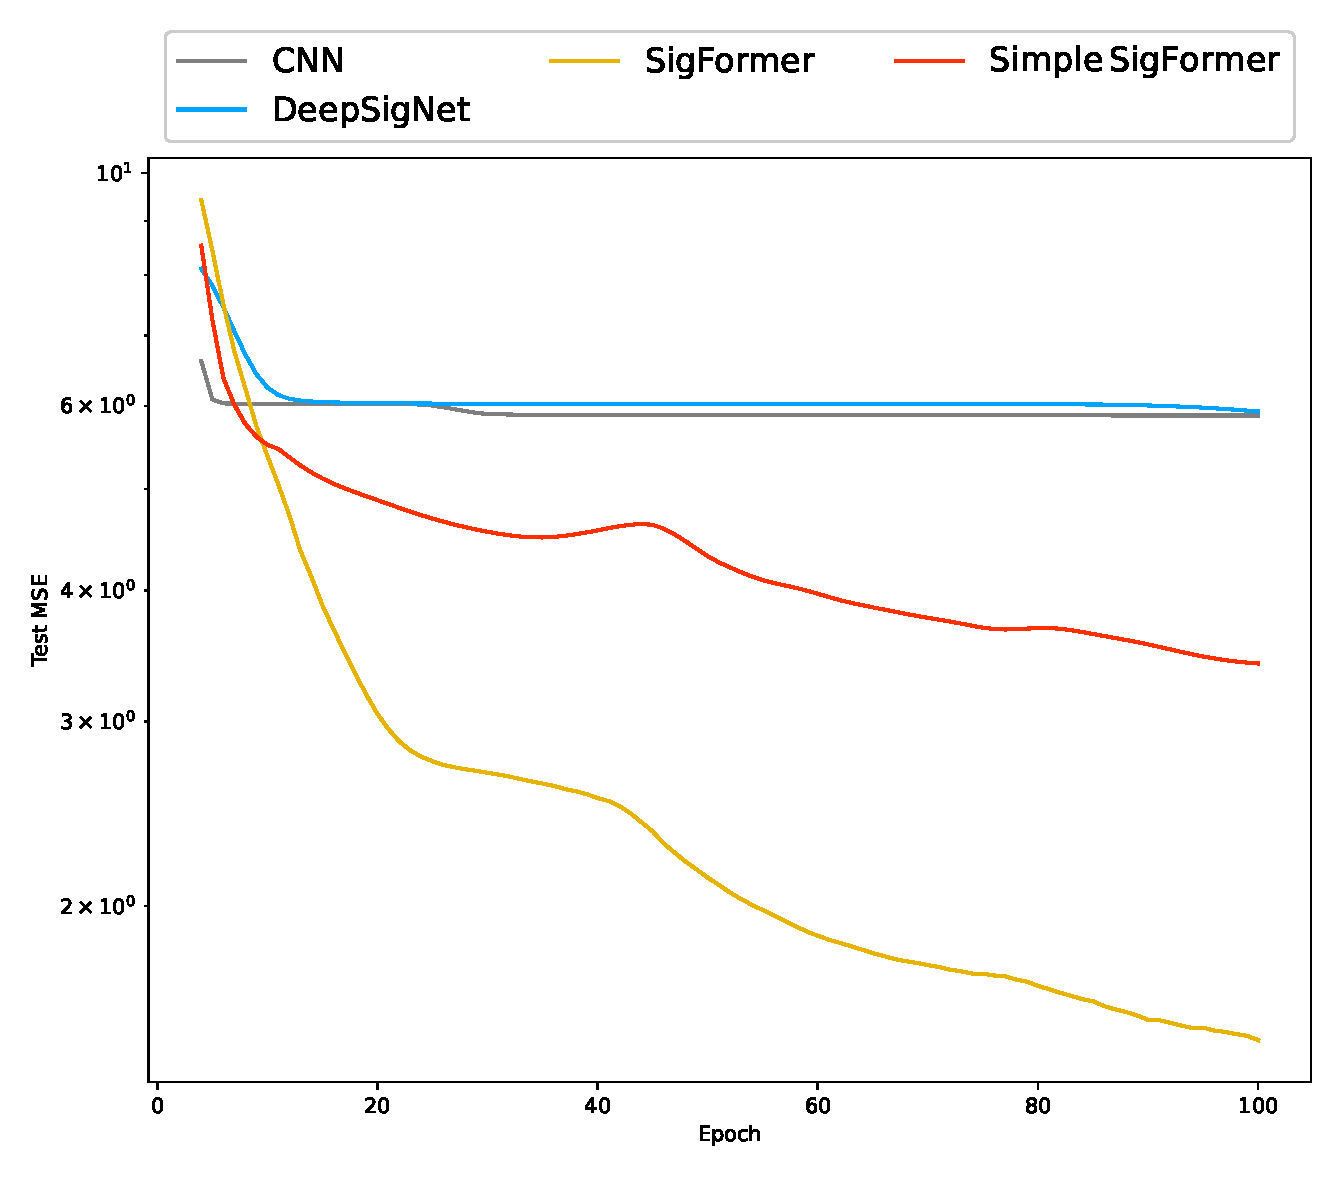
\includegraphics[width=0.45\textwidth]{fig//rHeston_grid=100_Hbeta_kappa1uniform_kappa2uniform_theta=0.3_v0=0.01.eps}
		
\includegraphics[width=0.45\textwidth]{fig//rHeston_grid=100_Hbeta_kappa1uniform_kappa2uniform_thetauniform_v0=0.01.eps}
		\caption{Loss plot of (Left:) three and (Right:) four parameters calibration for rHeston volatility processes with $H\sim\text{Beta}(1,\,9)$, $\kappa_1\sim\text{Uniform}(0,\,5)$, $\kappa_2\sim\text{Uniform}(0,\,3)$ and $\theta\sim\text{Uniform}(0,0.5)$. The data has been taken the rolling mean with a window size of 5.}
	\end{figure}
	
	
	
	\subsection{Loss plots for the SigFormer model with different complexities}
	\label{subapdix-loss-plots-complexity}
	\begin{figure}[H]
		\centering
		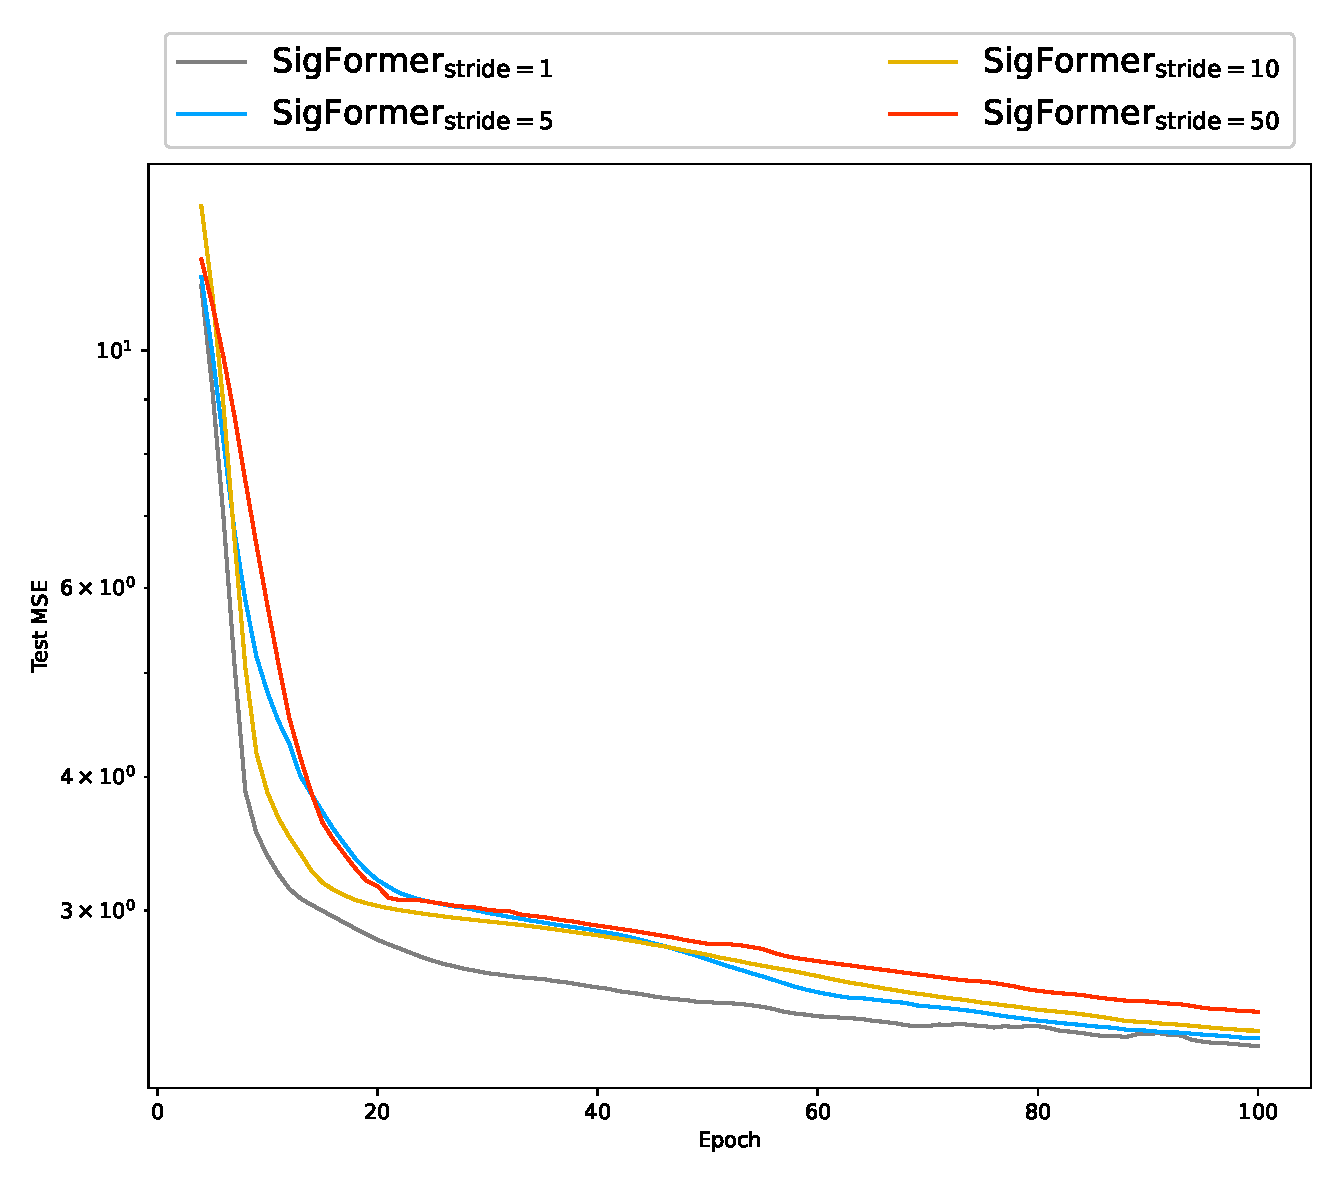
\includegraphics[width=0.8\textwidth]{fig//rHeston_grid=100_Hbeta_kappa1uniform_kappa2uniform_thetauniform_v0=0.01_diffstride.eps}
		\caption{Loss plot for the SigFormer model with the stride varying from $1$ to $50$. Here $H\sim\text{Beta}(1,\,9)$, $\kappa_1\sim\text{Uniform}(0,\,5)$, $\kappa_2\sim\text{Uniform}(0,\,3)$, $\theta\sim\text{Uniform}(0,\,0.5)$ and the input lengths equal to $100$. The data has been taken the rolling mean with a window size of 5.}
	\end{figure}
\end{document}
